\section{Momentenregelung des Antriebstranges} \label{regelung}
%Chris
\subsection{Regelungsziele und Regelkreis} \label{regelziel}
Bevor eine Regelung für die WEA umgesetzt werden kann, müssen zunächst einige Regelungsziele festgelegt werden. Aus der Beschreibung der Regelungsziele ergeben sich die Regelanforderungen der WEA. Des Weiteren wird die Komplexität des Reglers durch ein geeignetes Funktionsmodell, welches das dynamische Verhalten der Regelstrecke bestimmt, beschrieben. Hierfür wird das torsionsstarre Triebstrangmodell verwendet. Die Regelung konzentiert sich auf die Einhaltung und Umsetzung der Hauptziele, wobei das Verhalten der Blätter, des Turms und des Antriebsstranges nicht berücksichtigt werden. Folglich reicht ein sehr vereinfachtes Funktionsmodell aus. Aus der Generatorcharakteristik lassen sich insgesamt drei Arbeitsbereiche ermitteln, nämlich der untere und obere Teillastbereich, sowie der Volllastbereich. Die folgende \autoref{tab:Tabelle4.1} fasst die Hauptziele des Reglers zusammen. Auf Grundlage dessen, werden in den folgenden Kapiteln die benötigten Regler für die verschiedenen Arbeitsbereiche entwickelt.
\\


\begin{table}[H]
    \centering
    \begin{tabular}{|l|}
        \hline                                                        
        \rowcolor{lightGrey}
        \multicolumn{1}{|c|}{ \textbf{Unterer Teillastbereich (I)}}                                                                                                   \\ \hline
    
         Leistungsoptimierung - Leistungsbeiwert \acs{cP} stets auf maximalen Leistungsbeiwert\\ \acs{cPmax} halten.
         \\
         Anforderung: \acs{cP} = \acs{cPmax}
                                   \\ \hline
        \rowcolor{lightGrey}
        \multicolumn{1}{|c|}{\textbf{Oberer Teillastbereich (II)}}                                                                                                      \\ \hline
        Leistungsoptimierung - Leistungsbeiwert \acs{cP} kleiner als maximaler Leistungsbeiwert\\ \acs{cPmax}.
        \\
        Anforderung: \acs{cP} < \acs{cPmax}
                                        \\ \hline
        \rowcolor{lightGrey}
        \multicolumn{1}{|c|}{\textbf{Volllastbereich (III)}}                                                                                                          \\ \hline
        Leistungsbegrenzung - Leistungsbeiwert \acs{cP} für eine konstante Entnahme der \\Nennwindleistung beeinflussen.
        \\
        Anforderung: \acs{cP} \ll \space \acs{cPmax}
        \\ \hline
    \end{tabular}
    \caption{Hauptziele des Reglers für die jeweiligen Arbeitsbereiche}
    \label{tab:Tabelle4.1}
\end{table}

Für die Regelung der WEA wird von einem Standardregelkreis ausgegangen, wie in \autoref{fig:Abbildung4.1} dargestellt. Wobei für den unteren Teillastbereich ein anderes Konzept verwendet wird und an sich keinen Standardregelkreis darstellt, was in Kapitel 4.2 noch genauer beschrieben wird.
\\
Als Stellgröße u eignet sich das Generatormoment \acs{MG} und der Pitchwinkel \acs{theta}. Da die Windgeschwindigkeit nur sehr ungenau messtechnisch erfasst werden kann und ein stochastisches Verhalten aufweist, eignet sich diese Größe als Störgröße z. Hingegen kann die Rotordrehzahl \acs{nR} sehr gut messtechnisch erfasst werden, da die Rotorblätter als Anemometer dienen. Daher eignet sich diese Größe gut als Führungs- und Regelgröße w und y. Die Regler- und Streckenübertragungsfunktionen des Führungs- und Störverhaltens werden für den oberen Teillastbereich und Volllastbereich separat mithilfe der Superposition ermittelt. Für die Regelung des Generatormomentes \acs{MG} im oberen Teillastbereich und für die Regelung des Pitchwinkels \acs{theta} im Volllastbereich wird lediglich das Führungsverhalten betrachtet.

\begin{figure}[H]
    \centering
    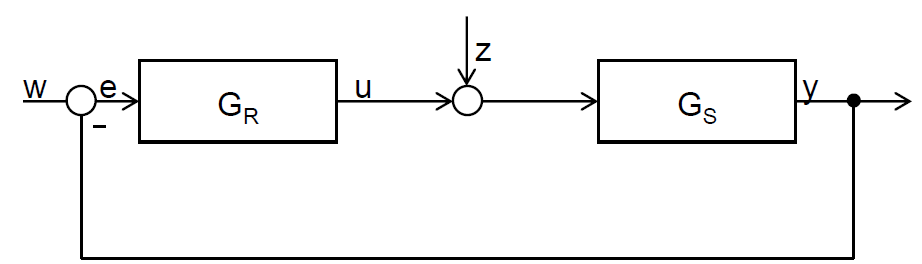
\includegraphics[scale=0.45]{Bilder/Kapitel 6/Standardregelkreis.PNG}
    \caption{Standardregelkreis}
    \label{fig:Abbildung4.1}
\end{figure}

%Chris
\subsection{Unterer Teillastbereich}

Laut \autoref{tab:Tabelle4.1} ist für den unteren Teillastbereich eine Leistungsoptimierung notwendig, da die Windleistung \acs{PW} unterhalb der Generatornennleistung \acs{PGNenn} liegt. Die Rotordrehzahl \acs{nR} liegt folglich noch unter der Generatornenndrehzahl \acs{nGNenn}, wodurch diese noch variabel an die Windgeschwindigkeit \acs{v1} angepasst werden kann. Dies wird mithilfe des bremsend wirkenden Generatormomentes \acs{MG} erreicht. Aufgrund dessen ergibt sich ein optimales Anströmverhältnis und es resultiert ein maximaler Leistungsbeiwert. Im unteren Teillastbereich kann mit steigender Windgeschwindigkeit also die maximal mögliche Windleistung entnommen werden, das heißt, der Leistungsbeiwert \acs{cP} wird stets auf den maximalen Leistungsbeiwert \acs{cPmax} geregelt.
\\
Für die Herleitung des Regelkreises wird von einer nicht linearen Bewegungs-DGL des torsionsstarren Triebstrangs ausgegangen. Der Vorteil für die Reglerauslegung im unteren Teillastbereich besteht darin, dass von der nicht linearen Bewegungs-DGL aus einer Leistungsbilanz ein Regelgesetz abgeleitet wird, welches einen Zusammenhang zwischen Regel- und Stellgröße darstellt. Durch das Regelgesetz wird mithilfe des berechneten Generatormoments \acs{MG} eine stationäre Rotordrehzahl \acs{omegaR} eingestellt. Es wird für diese Methode keine Führungsgröße benötigt. Dies vereinfacht die Entwicklung des Regelkreises für den unteren Teillastbereichs deutlich, da keine genaue Kenntnis der Steckenübertragungsfunktion nötig ist. Daher kann der untere Teillastbereich nicht als Standardregelkreis betrachtet werden. Dieses \glqq Steuerungskonzept\grqq{} zur Regelung des unteren Teillastbereiches hat sich als Standardmethode für diesen Arbeitsbereich durchgesetzt. Das Regelgesetz für die Stellgröße \acs{MG} wird mit folgenden Gleichungen beschrieben:

\begin{align}
    \acs{MG}(\acs{omegaG}) = k_I \cdot \acs{omegaR}^2 \enspace ,wobei \enspace \acs{kI} = const.
    \label{eq:Gleichung4.1}
\end{align}

mit:

\begin{align}
   \acs{kI} = \frac{1}{2} \cdot \rho \cdot \pi \cdot R^5 \cdot \frac{1}{\acs{lambdaopt}^3} \cdot \frac{1}{\acs{ng}} \cdot \acs{cP}(\acs{lambdaopt})
   \label{eq:Gleichung4.2}
\end{align}
\newline
Der Vorteil bei diesem Steuerungskonzept besteht nun darin, dass für jede Änderung der Windgeschwindigkeit \acs{v1} ein neuer stationärer Arbeitspunkt mit stationärer Rotorwinkelgeschwindigkeit \acs{omegaR} entsteht. Dabei ergibt sich ein entsprechendes Generatormoment \acs{MG}, welches mithilfe der \autoref{eq:Gleichung4.1} und \autoref{eq:Gleichung4.2} berechnet wird. Das heißt, zu jeder Windgeschwindigkeit wird das zugehörige Generatormoment \acs{MG} zugeordnet, wodurch die Notwendigkeit eines PI(D)-Reglers entfällt.
\\
Die Rotorwinkelgeschwindigkeit \acs{omegaR} wird stets optimal an die Windgeschwindigkeit angepasst. Es besteht für stationäre Arbeitspunkte ein eindeutiger Zusammenhang zwischen Rotordrehzahl \acs{omegaR} und der Windgeschwindigkeit \acs{v1}. Die optimale Schnelllaufzahl \acs{lambdaopt} kann im voraus berechnet werden und ist für den unteren Teillastbereich konstant. Aufgrund dessen, wird mithilfe der \autoref{eq:Gleichung4.3}, aus der Rotorwinkelgeschwindigkeit und konstanten Schnelllaufzahl die zugehörige Windgeschwindigkeit \acs{v1} berechnet.  Damit ergibt sich für den Leistungsbeiwert \acs{cP} ein optimaler Leistungsbeiwert \acs{cPopt}, jedoch für den Momentenbeiwert \acs{cM} kein optimaler Momentenbeiwert \acs{cMopt}. Aus der Formulierung der Regelziele ergab sich eine Leistungsoptimierung für den unteren Teillastbereich, sodass der Leistungsbeiwert \acs{cP} auf einen optimalen Wert geregelt werden muss, da erst so die maximale Entnahme der Windleistung \acs{PW} entsteht. Daher wird das Erreichen eines optimalen Momentenbeiwertes \acs{cMopt} nicht angestrebt, da die Leistungsoptimierung durch Drehzahlanpassung stattfindet.   

\begin{align}
    \acs{v1} = \frac{\acs{omegaR} \cdot {R}}{\acs{lambdaopt}} \enspace ,wobei \enspace \acs{lambda} = \acs{lambdaopt}
    \label{eq:Gleichung4.3}
\end{align}
\newline
Die Steuerung für den unteren Teillastbereich wird als Funktionsblock in Matlab Simulink implementiert. In diesem Block wird der Faktor \acs{kI} berechnet und hinterher mit der Rotorwinkelgeschwindigkeit $\acs{omegaR}^2$ multipliziert, um als Ergebnis eine Generatormomentsollwertvorgabe $M_{G,soll}$ für das Triebstrangmodell zu erhalten. Die \autoref{fig:Abbildung4.2} zeigt die Blockdarstellung der Steuerung inklusive der Ein- und Ausgansparameter.

\newpage

\begin{figure}[H]
   \centering
   \begin{pspicture}[showgrid=false](0,0)(10,5)
        \psframe(0,0)(10,5)
        % Modell
        \psframe[linecolor=black,fillcolor=lightGrey,fillstyle=solid](0.5,0.5)(4,4.5)
        \rput(2.25,2.8){\small Steuerung unterer}
        \rput(2.25,2.3){\small Teillastbereich}
        % Ausgänge Block
        \psline{->}(4,2.5)(6,2.5)
        \rput(5.5,2.9){\footnotesize \acs{kI}}
        %Multiplikation
        \psframe[linecolor=black,fillcolor=lightGrey,fillstyle=solid](6.0,0.5)(6.5,4.5)
        \rput(6.25,2.5){\small \cdot}
        % Eingang Multiplikation
        \psline{-}(4.5,4.5)(4.5,3.5)
        \psline{->}(4.5,3.5)(6,3.5)
        \rput(5.3,4.5){\footnotesize {\acs{omegaR}$^2$}}
        % Ausgang Multiplikation
        \psline{->}(6.5,2.5)(9,2.5)
        \rput(8.5,2.9){\footnotesize \acs{MG}}
    \end{pspicture}
   \caption[Übersicht Steuerung unterer Teillastbereich]{Blockdarstellung der Steuerung des unteren Teillastbereichs inklusive der Ein- und Ausgangsparameter}
   \label{fig:Abbildung4.2}
\end{figure}

%Chris
\subsection{Linearisierung der Streckenübertragungsfunktion}
Für die Reglerauslegung im oberen Teillastbereich und Vollastbereich müssen zunächst die Streckenübertragungsfunktionen ausgehend vom torsionsstarren Antriebstrangmodell und der daraus resultierenden nichtlinearen Bewegungs-DGL linearisiert werden. Aus dem Ergebnis der Linearisierung entstehen sogenannte Linearisierungskoeffizienten, welche für bestimmte stationäre Arbeitspunkte zugeordnet sind. Für den oberen Teillastbereich und dem Volllastbereich werden zunächst jeweils drei stationäre Arbeitspunkte mit den entsprechenden Linearisierungskoeffizienten betrachtet. Die Linearisierung erfolgt mittels der Taylorreihenentwicklung. Aus dem Funktionsmodell ergibt sich mit \autoref{eq:Gleichung4.4} die nichtlineare Bewegugns-DGL des Antriebstrangs, welche bereits im Kapitel 3 ausführlich diskutiert wurde. 

\begin{align}
    \ddot\varphi_R = \frac{1}{J} \cdot (\acs{MR} - \acs{ng} \cdot \acs{MG})
    \label{eq:Gleichung4.4}
\end{align}
\newline
Mithilfe der Taylorreihenentwicklung um einen stationären Arbeitspunkt \acs{omegaR} und lösen der nichtlinearen Bewegungs-DGL mit der Laplacetransformation ergibt sich folgende \autoref{eq:Gleichung4.5}, wobei sich insgesamt vier Linearisierungskoeffizienten ergeben, bei dem der Koeffizient bezogen auf das Generatormoment \acs{MG} nicht benötigt wird und daher nicht weiter aufgeführt ist.
\begin{align}
    \acs{omegaR} &= \frac{1}{J \cdot s - k_{\omega\mathrm{R}}} \cdot (\acs{kv} \cdot v + \acs{ktheta} \cdot \theta - \acs{ng} \cdot \acs{MG})\label{eq:Gleichung4.5}
    \enspace,wobei\\
    k_{\omega\mathrm{R}} &:= \left(\frac{\delta \acs{MR}}{\delta v}\right)_c , \enspace \acs{kv} := \left(\frac{\delta \acs{MR}}{\delta \omega_{\mathrm{R}}}\right)_c, \enspace  \acs{ktheta} := \left(\frac{\delta \acs{MR}}{\delta \theta}\right)_c  \nonumber
\end{align}
\newline
Zur Berechnung der Linearisierungskoeffizienten muss nun die Berechnungsvorschrift für das Rotormoment \acs{MR} aus \autoref{eq:Gleichung2.39} partiell abgeleitet werden, wobei der Momentenbeiwert \acs{cM} ebenfalls partiell nach \acs{lambda} und $\theta$ abgeleitet werden muss. Daraus ergeben sich die folgenden Gleichungen.

\begin{align}
    k_{\omega\mathrm{R,II(I),i}} &\approx \left(\frac{1}{2} \cdot \rho \cdot \acs{v1}^2 \cdot \pi \cdot \acs{R}^3 \cdot \left(\frac{\acs{R}}{\acs{v1}} \cdot \frac{\delta \acs{cM}_{,II(I),i}\left(\acs{lambda}\left(v,\acs{omegaR}\right),\theta\right)}{\delta \acs{lambda}}\right)\right)_c\label{eq:Gleichung4.6}\\
     \acs{kv}_{,II(I),i} &\approx \left(\frac{1}{2} \cdot \rho \cdot \acs{v1}^2 \cdot \pi \cdot \acs{R}^3 \cdot \left(2 \cdot \acs{v1} \cdot \acs{cM}_{,II(I),i}\left(\acs{lambda}\left(v,\acs{omegaR}\right),\theta\right) - \acs{omegaR} \cdot \acs{R} \cdot \frac{\delta \acs{cM}_{,II(I),i}\left(\acs{lambda}\left(v,\acs{omegaR}\right),\theta\right)}{\delta \acs{lambda}}\right)\right)_c\label{eq:Gleichung4.7}\\
    \acs{ktheta}_{,III,i} &\approx \left(\frac{1}{2} \cdot \rho \cdot \acs{v1}^2 \cdot \pi \cdot \acs{R}^3 \cdot \left(\frac{\delta \acs{cM}_{,III,i}\left(\acs{lambda}\left(v,\acs{omegaR}\right),\theta\right)}{\delta \acs{lambda}}\right)\right)_c\label{eq:Gleichung4.8}
\end{align}
\newline
Im Folgenden werden die weiteren nötigen Schritte aufgeführt, um die Berechnung der Linearisierungskoeffizienten zu vervollständigen. Zunächst berechnen sich die zugehörigen Schnelllaufzahlen \acs{lambda} für die Arbeitsbereiche und dessen stationäre Arbeitspunkte mit der \autoref{eq:Gleichung4.9}.

\begin{align}
    \acs{lambda}_{,II(I),i} = \frac{\acs{omegaR} \cdot R}{\acs{v1}_{,II(I),i}}
    \label{eq:Gleichung4.9}
\end{align}
\newline
Hinterher werden die partiellen Ableitungen der Momentenbeiwerte \acs{cM} mithilfe der \autoref{eq:Gleichung4.10} und Unterscheidung der Arbeitsbereiche berechnet. Für den oberen Teillastbereich muss die partielle Ableitung nach $\theta$ nicht erfolgen, da der Pitchwinkel hier Null beträgt. Der Pitchwinkel wird erst beim Volllastbereich von Bedeutung sein, wenn es darauf ankommt, die Rotordrehzahl \acs{nR} mithilfe des Pitchwinkels zu begrenzen.
\begin{align}
    \acs{cM}(\acs{lambda})_{,II(I),i,\theta} &= c_1 \cdot (1 + c_2 \cdot \sqrt{\theta + c_3}) + \frac{c_4}{\acs{lambda}}   \cdot (c_5 \cdot \acs{lambda}_i - c_6 \cdot \theta - c_7 \cdot \theta^{c_8} - c_9) \cdot e^{-c_{10} \cdot \acs{lambda}_i}
    \label{eq:Gleichung4.10}\\\enspace ,mit\nonumber\\
    \acs{lambda}_i &= \frac{1}{\acs{lambda}_{,II(I),i} + 0,008 \cdot \theta} - \frac{0,035}{c_{11} + c_{12} \cdot \theta^3}
    \nonumber
\end{align}

{\renewcommand{\arraystretch}{2}%
\begin{table}[H]
    \centering
    \begin{tabular}{|c|c|c|c|}
        \hline
        c$_1$ = 0,005 & c$_2$ = 1,53 & c$_3$ = 0,5 & c$_4$ = 0,18\\\hline
        c$_5$ = 121 & c$_6$ = 27,9 & c$_7$ = 198 & c$_8$ = 2,36\\\hline
        c$_9$ = 5,74& c$_{10}$ = 11,35 & c$_{11}$ = 16,1 & c$_{12}$ = 201\\\hline
    \end{tabular}
\end{table}
}

Die Berechnung der Schnelllaufzahlen \acs{lambda}$_{,II(I),i}$ für den jeweiligen Arbeitsbereich und dessen stationären Arbeitspunkte, die Berechnung der partiellen Ableitungen für die Momentenbeiwerte \acs{cM}$_{,II(I),i}$, sowie die Berechnung der Linearisierungskoeffizienten und dessen partielle Ableitungen, finden in einem separaten Matlab-File statt und werden bevor die Simulation gestartet wird vorangehend einmalig für die stationären Arbeitspunkte berechnet und für die Berechnung der Reglerkoeffizienten für den oberen Teillastbereich und Volllastbereich zur Verfügung gestellt, welche ebenfalls vor Simulationsstart einmalig berechnet werden und hinterher als Array der Simulation übergeben und in entsprechende Lookup Tables gespeichert werden.

%chris + Aaron
\subsection{Oberer Teillastbereich}
Laut \autoref{tab:Tabelle4.1} ist für den oberen Teillastbereich ebenfalls eine Leistungsoptimierung notwendig, da die Windleistung \acs{PW} noch unterhalb oder gleich der Generatornennleistung \acs{PGNenn} ist. Sofern die Rotordrehzahl \acs{nR} gleich der Generatornenndrehzahl \acs{nGNenn} ist, ist es nicht mehr möglich diese an die Windgeschwindigkeit anzupassen. Dadurch ergibt sich ein schlechtes Anströmverhältnis was einen nicht optimalen Leistungsbeiwert \acs{cP} zur Folge hat. Es wird zwar nicht mehr das Leistungsmaximum aus der zur Verfügung stehenden Windleistung entnommen, dennoch wird eine Leistungssteigerung mit ansteigender Windgeschwindigkeit \acs{v1} durch eine geeignete Regelung erzielt.\\
Für die Reglerauslegung des oberen Teillastbereiches wird eine algebraische Auslegung im Frequenzbereich durchgeführt. Zur Erfüllung der Hauptziele werden nun sogenannte Reglerkoeffizienten aus den vorher berechneten Linearisierungskoeffizienten ermittelt, welche später eine Generatormomentsollwertvorgabe $M_{G,soll}$ für den Antriebsstrang darstellen. Zur Bestimmung der Reglerkoeffizienten wird ein Referenzmodell herangezogen, welches das zu erwartendene Systemverhalten der Hauptziele des Reglers widerspiegelt. Dieses Referenzmodell wird anschließend mit dem physikalischen Modell, basierend auf den physikalischen Vorbetrachtungen der WEA, verglichen und überprüft, ob das gewünschte und resultierende Modell das gleiche Systemverhalten aufweist. Dieses Verfahren ist für das Führungs- und Störverhalten anzuwenden, wobei für den weiteren Verlauf der Arbeit sich auf das Führungsverhalten des Systems fokussiert wird. Auf Grundlage dessen, wird mittels Koeffizientenvergleich die Reglerkoeffizienten algebraisch berechnet. Auf die Herleitungen soll nicht weiter eingegangen werden. Damit ergibt sich für die Berechnung der Reglerkoeffizienten im oberen Teillastbereich folgende Gleichungen:
\begin{align}
    k_{P,W,II} &= \frac{3 \cdot J}{T_{Aus} \cdot i_G}   \label{eq:Gleichung4.11}\\
    k_{I,W,II} &= \frac{3 \cdot k_{\omega\mathrm{R,II,i}}}{T_{Aus} \cdot i_G}\label{eq:Gleichung4.12}
\end{align}
\newline
In Matlab werden nun die Reglerkoeffizienten einmalig für jeden Arbeitspunkt im oberen Teillastbereich berechnet und der Simulation als Lookup-Table übergeben. Da es sich hierbei um einen Delta-Regler handelt, muss die Differenz aus Soll-Drehzahl und Ist-Drehzahl mit den Reglerkoeffizienten verrechnet werden. Die Auswahl der richtigen Reglerkoeffizienten im Lookup-Table wird durch das entsprechende Generatormoment \acs{MG} im jeweiligen Arbeitspunkt bestimmt. Der Regelkreis für den oberen Teillastbereich ist grundlegend der \autoref{fig:Abbildung4.3} zu entnehmen.

 \begin{figure}[H]
    \centering
    \fbox{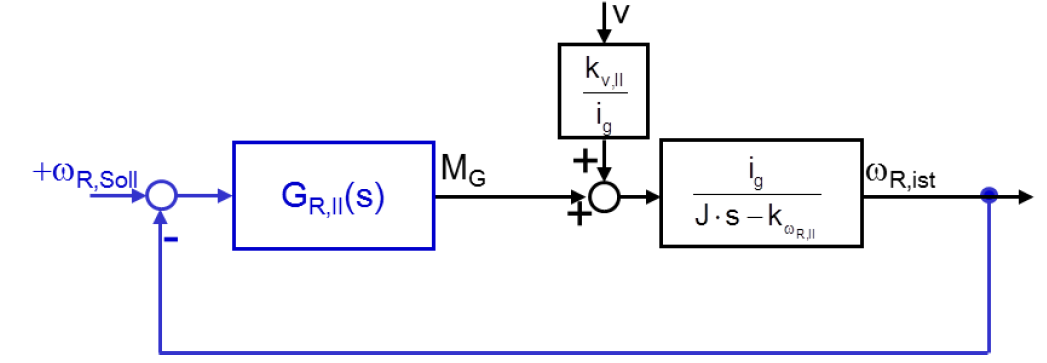
\includegraphics[width=0.9\textwidth]{Bilder/Kapitel 5/Führungsübertragungsfunktion_oberer_Teillastbereich.PNG}}
    \caption[Reglerkreis - oberer Teillastbereich]{Regelkreis - oberer Teillastbereich mit der Führungsübertragungsfunktion $G_{R,II}(s)$ \cite{SkriptSchulte}}
    \label{fig:Abbildung4.3}
\end{figure}

\subsection{Volllastbereich}
Laut \autoref{tab:Tabelle4.1} ist für den Volllastbereich eine Leistungsbegrenzung vorzusehen, da nun die Windleistung \acs{PW} oberhalb der Generatornennleistung \acs{PGNenn} liegt. Durch das Pitchen der Blätter wird bewusst das Anströmverhältnis verschlechtert, denn das Betreiben der WEA darf nicht weit über Nenndrehzahl erfolgen. Dies führt zur Beschädigung oder gar Zerstörung der WEA. Das Pitchen ermöglicht jedoch bei ansteigender Windleistung (\acs{PW} > \acs{PGNenn}) weiterhin eine konstante Generatornennleistung \acs{PGNenn} zu erzielen. Der Pitchwinkel \acs{theta} spielt nun für die Reglerauslegung eine entscheidene Rolle.\\
Das Vorgehen zur Bestimmung der Reglerkoeffizienten ist gleich dem Vorgehen aus dem oberen Teillastbereich. Das Verfahren ist hier ebenfalls auf das Führungs- und Störverhalten anzuwenden, jedoch wird beim Volllastbereich lediglich das Führungsverhalten betrachet. Die folgenden Gleichungen zeigen die Berechnungen der entsprechenden Reglerkoeffizienten. Der Unterschied hier ist, das der P- und I-Anteil des Reglers von $k_\theta$ abhängig ist. Im Volllastbereich gilt es den Pitchwinkel so zu regeln, dass das Generatormoment \acs{MG} = const. bleibt.

\begin{align}
    k_{P,W,III} &= \frac{3 \cdot J}{T_{Aus} \cdot k_\theta}   \label{eq:Gleichung4.13}\\
    \nonumber\\
    k_{I,W,III} &= \frac{3 \cdot k_{\omega\mathrm{R,III,i}}}{T_{Aus} \cdot k_\theta}\label{eq:Gleichung4.14}
\end{align}
\newline
Auch hier werden die Reglerkoeffizienten einmalig für jeden stationären Arbeitspunkt berechnet und der Simulation als Lookup-Table übergeben. Die Funktionsweise und Vorgehensweise ist dabei die Gleiche, wie beim oberen Teillastbereich, wobei die Auswahl der Reglerkoeffizienten anhand des einzustellenden Pitchwinkels erfolgt. Die \autoref{fig:Abbildung4.4} zeigt den grundlegenden Aufbau des Regelkreises für den Volllastbereich.

\begin{figure}[H]
    \centering
    \fbox{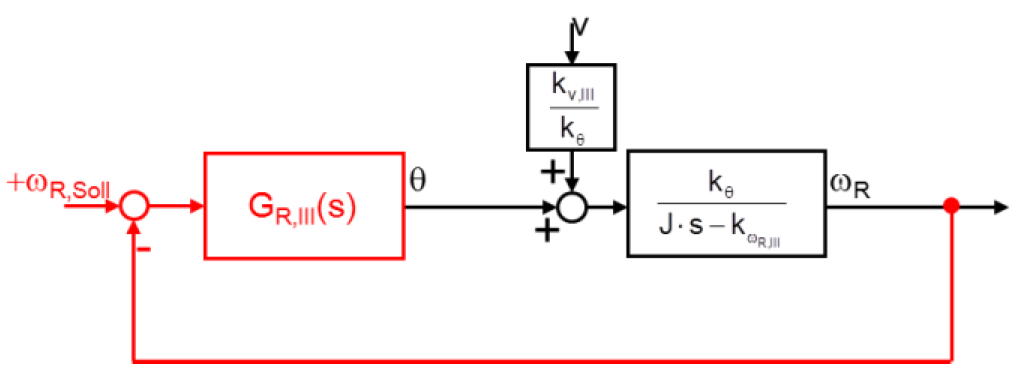
\includegraphics[width=0.9\textwidth]{Bilder/Kapitel 5/Führungsübertragungsfunktion_Volllastbereich.PNG}}
    \caption[Reglerkreis - Volllastbereich]{Regelkreis - Volllastbereich mit der Führungsübertragungsfunktion $G_{R,III}(s)$ \cite{SkriptSchulte}}
    \label{fig:Abbildung4.4}
\end{figure}

%Aaron
\subsection{Zustandsautomat} \label{statemachine}

Wie bereits in \autoref{regelziel} erläutert wurde, wird die Windenergieanlage in Abhängigkeit von der Windgeschwindigkeit \acs{v1} \bzw der Rotorwinkelgeschwindigkeit \acs{omegaR} in verschiedenen Lastbereichen mit ihren eigenen Regelzielen geregelt. Der Betrieb und damit auch die Regelung der Gesamtanlage bedarf folglich der Integration der in den vorangegangenen Unterabschnitten entworfenen Regler in eine Gesamtstruktur. \autoref{fig:Abbildung4.5} zeigt auf der linken Seite die Steuereinheit des unteren Teillastbereiches sowie die PI-Regler für den oberen- und den Volllastbereich. Da insbesondere die Regler nur für ihren jeweiligen Arbeitsbereich ausgelegt sind, ist es erforderlich deren Integratoren zurückzusetzen, wenn ein Lastbereich verlassen wird. Ebenfalls bedarf es einer Implementierung einer Sicherheitsabschaltung bei zu großen Windgeschwindigkeiten. Beide Aufgaben werden von einem Zustandsautomaten erfüllt, welcher in Simulink als Function-Block über die Nutzung einer Switch-Case-Anweisung implementiert wurde. Besagter Zustandsautomat ist in \autoref{fig:Abbildung4.5} auf der rechten Seite zu erkennen. Der Zustandsautomat erhält die Regelgrößen \acs{MG} für die beiden Teillastbereiche und \acs{theta} für den Vollastbereich, sowie die Ist-Winkelgeschwindigkeit des Rotors \acs{omegaRist} und die aktuelle Windgeschwindigkeit \acs{v1}. Von dem Zustandsautomaten werden die Sollwerte für \acs{MG} \bzw \acs{theta} und die Rücksetzbedingungen der beiden Integratoren in den PI-Reglern ausgegeben. 

\begin{figure}[H]
   \centering
   \begin{pspicture}[showgrid=false](0,0)(12,9.5)
        \psframe(0,0)(12,9.5)
        % UTLB
        \psframe[linecolor=black,fillcolor=lightGrey,fillstyle=solid](0.5,0.5)(4.5,2.5)
        \rput(2.5,1.75){\small Regler}
        \rput(2.5,1.25){\small Volllastbereich}
        % OTLB
        \psframe[linecolor=black,fillcolor=lightGrey,fillstyle=solid](0.5,3)(4.5,5)
        \rput(2.5,4.25){\small Regler oberer}
        \rput(2.5,3.75){\small Teillastbereich}
        % VLB
        \psframe[linecolor=black,fillcolor=lightGrey,fillstyle=solid](0.5,5.5)(4.5,7.5)
        \rput(2.5,6.75){\small Steuerung unterer}
        \rput(2.5,6.25){\small Teillastbereich}
        % Statemachine
        \psframe[linecolor=black,fillcolor=lightGrey,fillstyle=solid](6.5,0.5)(10,9)
        \rput(8.25,5.25){\small Zustands-}
        \rput(8.25,4.75){\small automat}
        % Regler -> Statemachine
        \psline{->}(4.5,1.5)(6.5,1.5)
        \rput(5.5,1.8){\footnotesize \acs{theta3}}
        \psline{->}(4.5,4)(6.5,4)
        \rput(5.5,4.3){\footnotesize \acs{MG2}}
        \psline{->}(4.5,6.5)(6.5,6.5)
        \rput(5.5,6.8){\footnotesize \acs{MG1}}
        % -> Statemachine
        \psline{-}(5.5,9)(5.5,8.5)
        \psline{->}(5.5,8.5)(6.5,8.5)
        \rput(5.2,8.75){\footnotesize \acs{v1}}
        \psline{->}(2.5,8)(6.5,8)
        \rput(3.5,8.3){\footnotesize \acs{omegaRist}}
        % Statemachine ->
        \psline{->}(10,8)(11.5,8)
        \rput(10.75,8.3){\footnotesize \acs{MGsoll}}
        \psline{->}(10,5.827)(11.5,5.827)
        \rput(10.75,6.127){\footnotesize \acs{thetasoll}}
        \psline{->}(10,3.66)(11.5,3.66)
        \rput(10.75,3.96){\footnotesize $Reset_{\mathrm{II}}$}
        \psline{->}(10,1.5)(11.5,1.5)
        \rput(10.75,1.8){\footnotesize $Reset_{\mathrm{III}}$}
    \end{pspicture}
   \caption[Regeleinheit der WEA]{Blockdarstellung der Regeleinheit der Windenergieanlage inklusive des Zustandsautomaten und der Regler für die drei Lastbereiche}
   \label{fig:Abbildung4.5}
\end{figure}

\autoref{fig:Abbildung4.6} zeigt das Zustandsdiagramm, welches in Simulink umgesetzt wurde. Gut im mittleren Bereich der Abbildung zu erkennen, sind die von \acs{omegaRist} abhängigen Übergangsbedingungen zwischen den Lastbereichen. Von entscheidender Relevanz für die Verhinderung der Zerstörung der WEA ist die Abschaltbedingung bei zu großen Winden ($v_1 > v_{\mathrm{1,krit}} = \SI{25}{\frac{m}{s}}$), welche in jedem Zustand berücksichtigt wird.

\begin{figure}[H]
    \centering
    \begin{pspicture}[showgrid=false](0,0)(15,18)
        \psframe(0,0)(15,18)
        
        % STATES
        % Idle State
        \Cnode[fillstyle=solid,fillcolor=lightGrey,radius=1cm](7.5,15.5){A}
        \rput(A){Idle}
        % UTLB
        \Cnode[fillstyle=solid,fillcolor=lightGrey,radius=1cm](12.5,11.5){B}
        \rput(B){UTLB $\mathrm{I}$}
        % OTLB
        \Cnode[fillstyle=solid,fillcolor=lightGrey,radius=1cm](7.5,7.5){C}
        \rput(C){OTLB $\mathrm{II}$}
        % VLB
        \Cnode[fillstyle=solid,fillcolor=lightGrey,radius=1cm](2.5,11.5){D}
        \rput(D){VLB $\mathrm{III}$}
        % E-Stop
        \Cnode[fillstyle=solid,fillcolor=lightGrey,radius=1cm](7.5,2.5){E}
        \rput(E){E-Stop}
        
        % VERBINDUNGEN
        % Start
        \psline{->}(5,15.5)(6.51,15.5)
        \rput*(5.5,15.8){\small$Start$}
        % Idle -> Idle
        \ncloop[angleB=105, angleA=75, loopsize=0, arm=0.5, linearc=0.2]{->}{A}{A}
        \ncput*{\small$else$}
        % Idle -> UTLB
        \nccurve[angleB=90, angleA=0]{->}{A}{B}
        \ncput*{\small$\omega_{\mathrm{r,ist}} \geq 0.3 \cdot \omega_{\mathrm{r,nenn}}$}
        % UTLB -> Idle
        \nccurve[angleB=-50, angleA=150]{->}{B}{A}
        \ncput*{\small$\omega_{\mathrm{r,ist}} < 0.25 \cdot \omega_{\mathrm{r,nenn}}$}
        % UTLB -> UTLB
        \ncloop[angleB=-15, angleA=15, loopsize=0, arm=0.5, linearc=0.2]{->}{B}{B}
        \ncput*{\small$else$}
        % UTLB -> OTLB
        \nccurve[angleB=0, angleA=-60]{->}{B}{C}
        \ncput*{\small$\omega_{\mathrm{r,ist}} \geq 0.9 \cdot \omega_{\mathrm{r,nenn}}$}
        % OTLB -> UTLB
        \nccurve[angleB=-120, angleA=30]{->}{C}{B}
        \ncput*{\small$\omega_{\mathrm{r,ist}} < 0.85 \cdot \omega_{\mathrm{r,nenn}}$}
        % OTLB -> OTLB
        \ncloop[angleB=-60, angleA=-30, loopsize=-0.4, arm=0.5, linearc=0.2]{->}{C}{C}
        \ncput*{\small$else$}
        % OTLB -> VLB
        \nccurve[angleB=70, angleA=60]{->}{C}{D}
        \ncput*{\small$\omega_{\mathrm{r,ist}} \geq \omega_{\mathrm{r,nenn}}$}
        % VLB -> OTLB
        \nccurve[angleB=120, angleA=0]{->}{D}{C}
        \ncput*{\small$\omega_{\mathrm{r,ist}} < 0.98 \cdot \omega_{\mathrm{r,nenn}}$}
        % VLB -> VLB
        \ncloop[angleB=165, angleA=195, loopsize=0, arm=0.5, linearc=0.2]{->}{D}{D}
        \ncput*{\small$else$}
        % UTLB -> E-Stop
        \nccurve[angleB=0, angleA=-45]{->}{B}{E}
        \ncput*{\small$v_1 > v_{1,\mathrm{krit}}$}
        % OTLB -> E-Stop
        \nccurve[angleB=90, angleA=-90]{->}{C}{E}
        \ncput*{\small$v_1 > v_{1,\mathrm{krit}}$}
        % VLB -> E-Stop
        \nccurve[angleB=180, angleA=-100]{->}{D}{E}
        \ncput*{\small$v_1 > v_{1,\mathrm{krit}}$}
        % Idle -> E-Stop
        \nccurve[angleB=130, angleA=-110]{->}{A}{E}
        \ncput*{\small$v_1 > v_{1,\mathrm{krit}}$}
        % E-Stop -> Idle
        \nccurve[angleB=-130, angleA=160]{->}{E}{A}
        \ncput*{\small$v_1 < 0.9 \cdot v_{1,\mathrm{krit}}$}
        % E-Stop -> E-Stop
        \ncloop[angleB=255, angleA=285, loopsize=0, arm=0.5, linearc=0.2]{->}{E}{E}
        \ncput*{\small$else$}
    \end{pspicture}
    \caption[Statemachine WEA]{Statemachine-Abbildung zur Darstellung der Lastbereiche und den jeweiligen Übergangsbedingungen}
    \label{fig:Abbildung4.6}
\end{figure}

%Aaron
\subsection{Reglervalidierung} \label{reglervalidierung}

Ziel dieses Unterabschnittes ist die Verifikation der erfolgreichen Umsetzung der Regelziele, die Funktionstüchtigkeit der Regler in Bezug auf die zuvor entwickelten Teilmodelle der Anlage und die Prüfung der Einhaltung der definierten Grenzen (Constraints) des Systems. Letztere können in \autoref{einfuehrung} nachgelesen werden. \\
Die Validierung der Regelung gliedert sich grundsätzlich in die Bereiche \glqq 4.7.1: Darstellung der Simulationsergebnisse\grqq{}, \glqq 4.7.2: Validierung der Regelziele\grqq{} und \glqq 4.7.3: Prüfung der Einhaltung der Constraints\grqq{}. Zunächst sollen generelle Zusammenhänge grafisch dargestellt und diskutiert werden. Daran anschließend wird geprüft, inwiefern sich die Ergebnisse mit den beschriebenen Regelzielen decken. Abschließend werden insbesondere die nicht eingehaltenen Grenzen des Systems auf ihre Ursache diskutiert. Im Ausblick (\autoref{ausblick}) werden mögliche Lösungsansätze für ermittelte Probleme kurz dargestellt.

\subsubsection{Darstellung der Simulationsergebnisse}

Das Modell der WEA inklusive der Steuerung/Regelung dieser wird gegen verschiedene Winde als Störgröße getestet. Auf die Prüfung des Führungsverhaltens wird an dieser Stelle verzichtet, da der Einfluss des Windes als Störgröße von größerer Bedeutung ist. Getestet werden soll das entwickelte System gegen:
\begin{enumerate}
    \item Winde mit konstanten Windgeschwindigkeiten
    \item Einzelne (IEC) Windböen
    \item Turbulente Winde
    \item Windgeschwindigkeitsstufen
\end{enumerate}

Dabei werden verschiedene Windgeschwindigkeiten beispielhaft simuliert. Begonnen werden soll mit dem Test des Modells gegen konstante Windgeschwindigkeiten. Windgeschwindigkeiten wurden hier so ausgewählt, dass die einzelnen Lastbereiche (Arbeitsbereiche) gut dargestellt werden können und Übergangsbedingungen klar zu erkennen sind.\\

\autoref{fig:Bild4.7} zeigt die Simulationsergebnisse für eine konstante Windgeschwindigkeit von $\SI{8}{\frac{m}{s}}$. In der oberen Abbildungshälfte dargestellt, werden die generatorseitige Winkelgeschwindigkeit und die Generatorleistung. An der Winkelgeschwindigkeit ist gut zu erkennen, dass durch die anliegende Windgeschwindigkeit der Rotor und damit auch der Generator beschleunigen, bis \ca zum Zeitpunkt \SI{90}{s} bei gegebenem Wind eine stationäre Geschwindigkeit erreicht wird. Die Winkelgeschwindigkeit stagniert bei rund einer Umdrehung pro Sekunde \bzw \SI{90}{\frac{rad}{s}}. Die Leistungskurve des Generators hat einen sehr ähnlichen Verlauf. Jedoch ist ein wesentlicher Unterschied im Bereich von $\SI{0}{s}$ bis $\SI{58}{s}$ zu erkennen. Erst ab $30\%$ der Nenndrehzahl des Rotors (vgl.\xspace \autoref{fig:Abbildung4.6} Zustand UTLB $\mathrm{I}$) setzt der untere Teillastbereich ein und damit auch die Ausgabe einer Leistung. Vorher befindet sich die Windenergieanlage noch im Leerlauf.

\begin{figure}[H]
   \centering
   \fbox{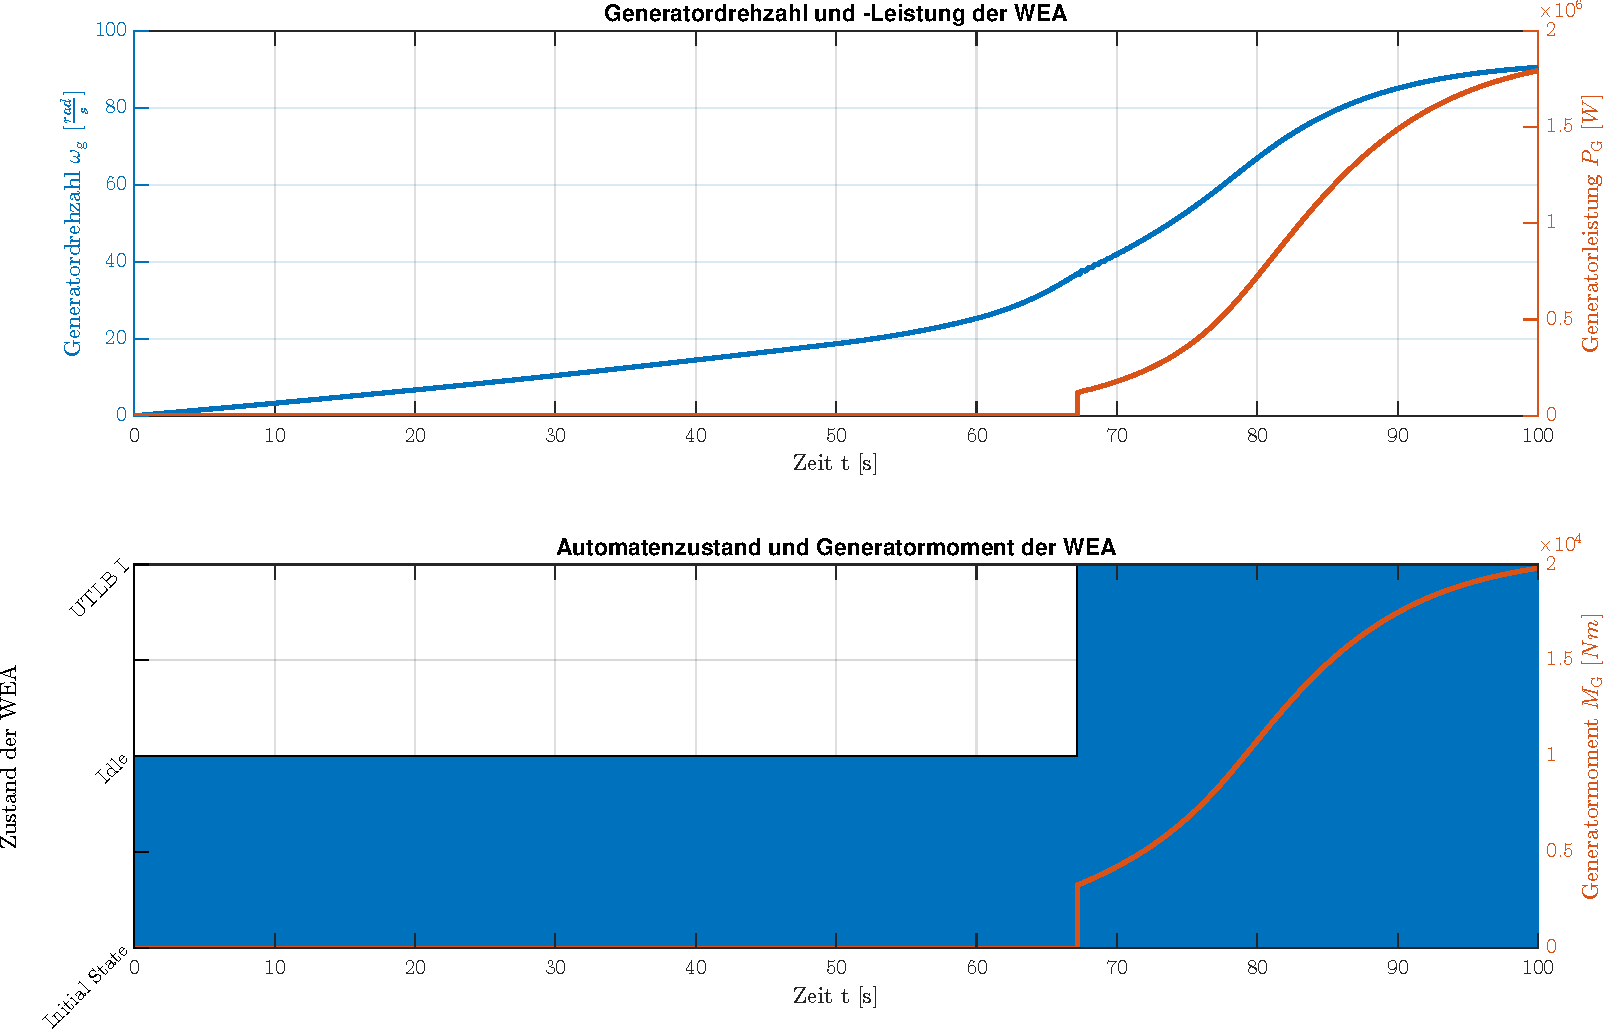
\includegraphics[width=1\textwidth]{Bilder/Kapitel 6/Reglervalidierung/const_wind_low.pdf}}
   \caption[Simulationsergebnisse langsamer konstanter Wind]{Simulationsergebnisse bei einem eingeprägten konstanten Wind von $\SI{9}{\frac{m}{s}}$}
   \label{fig:Bild4.7}
\end{figure}

In der unteren Hälfte von \autoref{fig:Bild4.7} zu erkennen ist der Zustand \bzw der Arbeitsbereich der Anlage sowie das generatorseitige Drehmoment. Da mit $\SI{9}{\frac{m}{s}}$ noch keine ausreichend hohe Rotordrehzahl erreicht wird, springt der Zustand lediglich vom Idle-Zustand in den unteren Teillastbereich. Ab dem Einsetzen des unteren Teillastbereiches liegt ein Moment am Generator an, welches aus dem rotorseitigen Moment resultiert. Auch das Moment steigt in einem ähnlichen Verlauf wie die Drehzahl an, bis zu dem Punkt, wo dem Wind die maximal mögliche Windleistung entnommen wird.\\

In \autoref{fig:Bild4.8} ist ein sehr ähnlicher Verlauf zu erkennen. In diesem Fall wurde mit einer Windgeschwindigkeit \acs{v1} von $\SI{10.7}{\frac{m}{s}}$ simuliert. In der oberen Hälfte ist die \ac{PG} und die Rotorwinkelgeschwindigkeit (\sim Rotordrehzahl) \ac{omegaG} erneut dargestellt. Die Leistung steigt nun bis knapp unter die Nennleistung an. Gleiches gilt auch für die Drehzahl. Die Leistung und das Generatordrehmoment setzen wie bereits zuvor bei $30\%$ der Nenndrehzahl ein.\\
Insbesondere ist in der unteren Hälfte der Abbildung die Einteilung der Kurven in die Last- \bzw Arbeitsbereiche ersichtlich. Bei \ca $\SI{69}{s}$ wird aufgrund des Erreichens von $90\%$ der Nenndrehzahl in den oberen Teillastbereich umgeschaltet. Die Umschaltbedingung geht aus \autoref{fig:Abbildung4.6} Zustand OTLB $\mathrm{II}$ hervor.

\begin{figure}[H]
   \centering
   \fbox{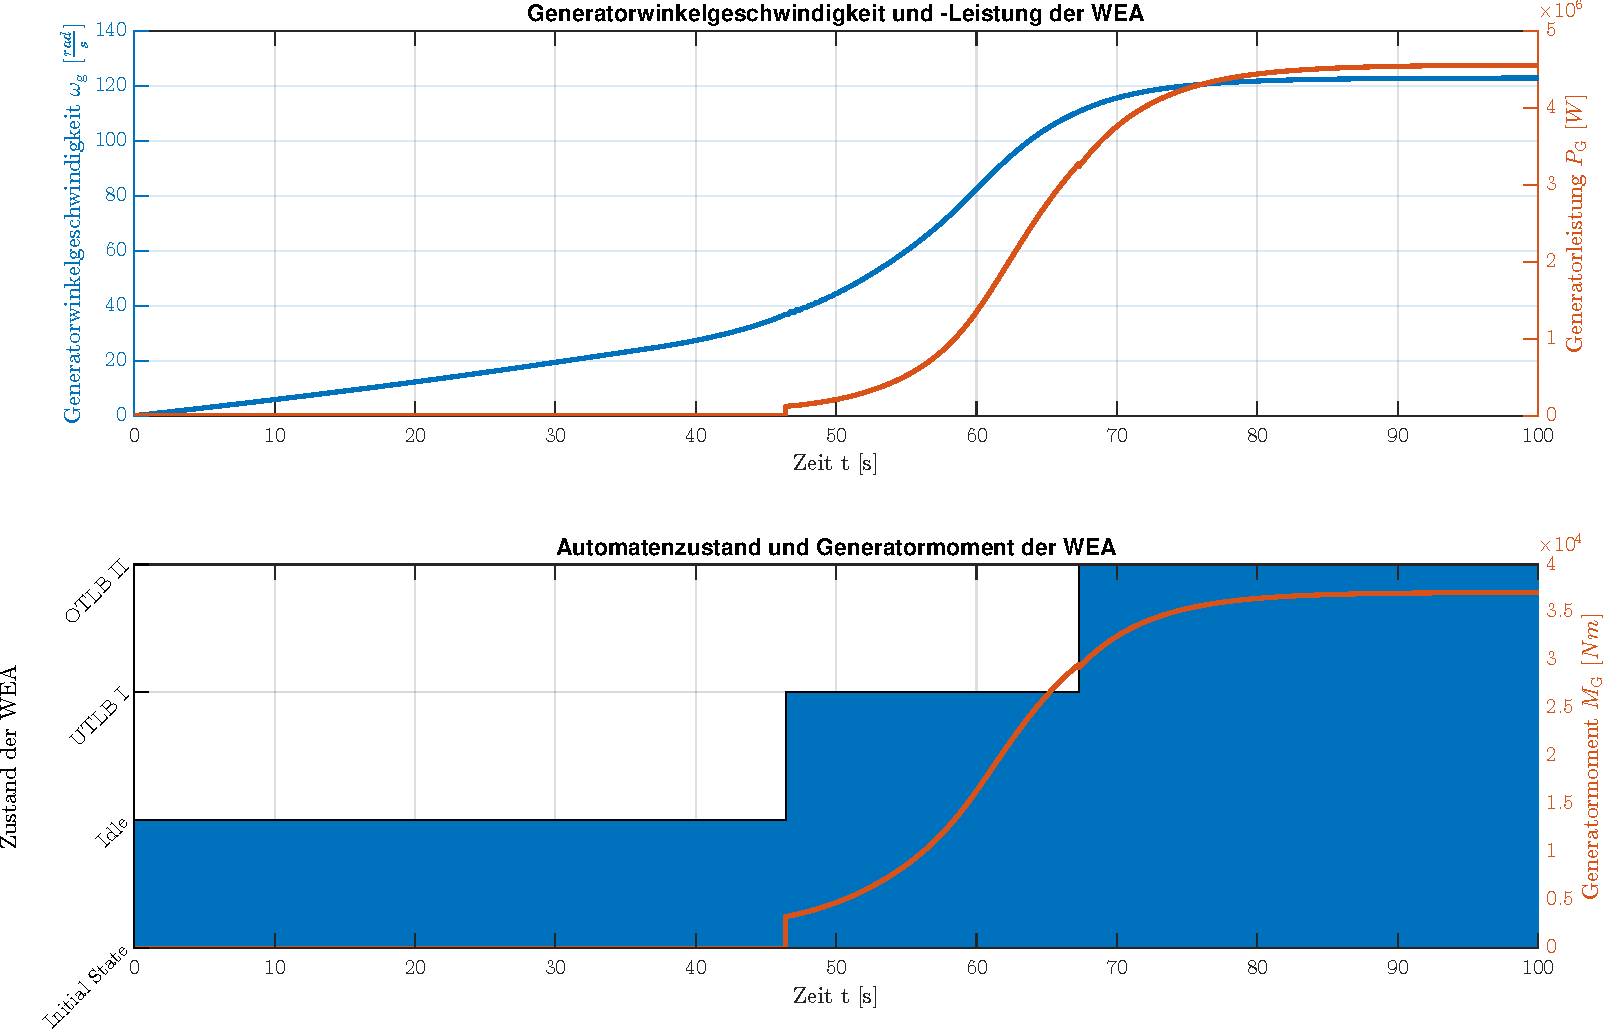
\includegraphics[width=1\textwidth]{Bilder/Kapitel 6/Reglervalidierung/const_wind_medium.pdf}}
   \caption[Simulationsergebnisse moderater konstanter Wind]{Simulationsergebnisse bei einem eingeprägten konstanten Wind von $\SI{10.7}{\frac{m}{s}}$}
   \label{fig:Bild4.8}
\end{figure}

Das letzte Diagramm aus der Reihe der konstanten Winde (\autoref{fig:Bild4.9}) bildet die Kurvenverläufe für einen Wind mit der Geschwindigkeit $\SI{14}{\frac{m}{s}}$ ab. Da der Wind nun stark genug ist, den Rotor bis zur Nenndrehzahl (und theoretisch auch darüber hinaus) zu beschleunigen, schaltet die Steuerung bis in den Volllastbereich hoch. Um die Nenngrößen für Drehzahl und Moment (\sim Leistung) konstant zu halten, müssen die Rotorblätter gepitched werden. Somit wurde ein weiterer Bereich in der Abbildung hinzugefügt, in welchem der \ac{theta} dargestellt wird.\\
Wenn man nun zunächst den oberen Teil der Grafik betrachtet, fällt auf, dass sowohl die Leistung als auch die Drehzahl leicht überschwingen, bevor sie auf dem Nennwert zurückfallen und nachfolgend konstant verlaufen. Grund dafür geht aus dem unteren Teil der Abbildung hervor. Der Pitchwinkel benötigt eine gewisse Zeit, bevor er seinen Sollwert erreicht hat. In dieser Zeit kommt es zu einer Überhöhung der Drehzahl und des Drehmoments auf der Rotorseite, welche wiederum auf die Generatorseite übertragen wird.\\
In der Mitte der Abbildung können erneut der aktuelle Arbeitsbereich und das Generatormoment abgelesen werden. Auch hier zeigt sich, dass bei \ca $\SI{51}{s}$ in den Vollastbereich umgeschaltet wird. Getriggert wird der Lastbereich durch das Erreichen der Nenndrehzahl (vgl.\xspace \autoref{fig:Abbildung4.6} Zustand VLB $\mathrm{III}$). Beim Generatormoment ist nun ebenfalls ein Unterschied zu den Teillastbereichen zu erkennen. Sobald die Nenndrehzahl erreicht wird, knickt das Moment sofort ab und verweilt konstant bei Nennmoment.\\
Der Pitchwinkel im unteren Bereich der Abbildung verweilt zunächst bis zum Umschalten in den Vollastbereich bei $0^\circ$. Erst dann steigt dieser mit $\SI{8}{\frac{^\circ}{s}}$ bis zum benötigten Pitchwinkel für die anliegende Windgeschwindigkeit an.

\begin{figure}[H]
   \centering
   \fbox{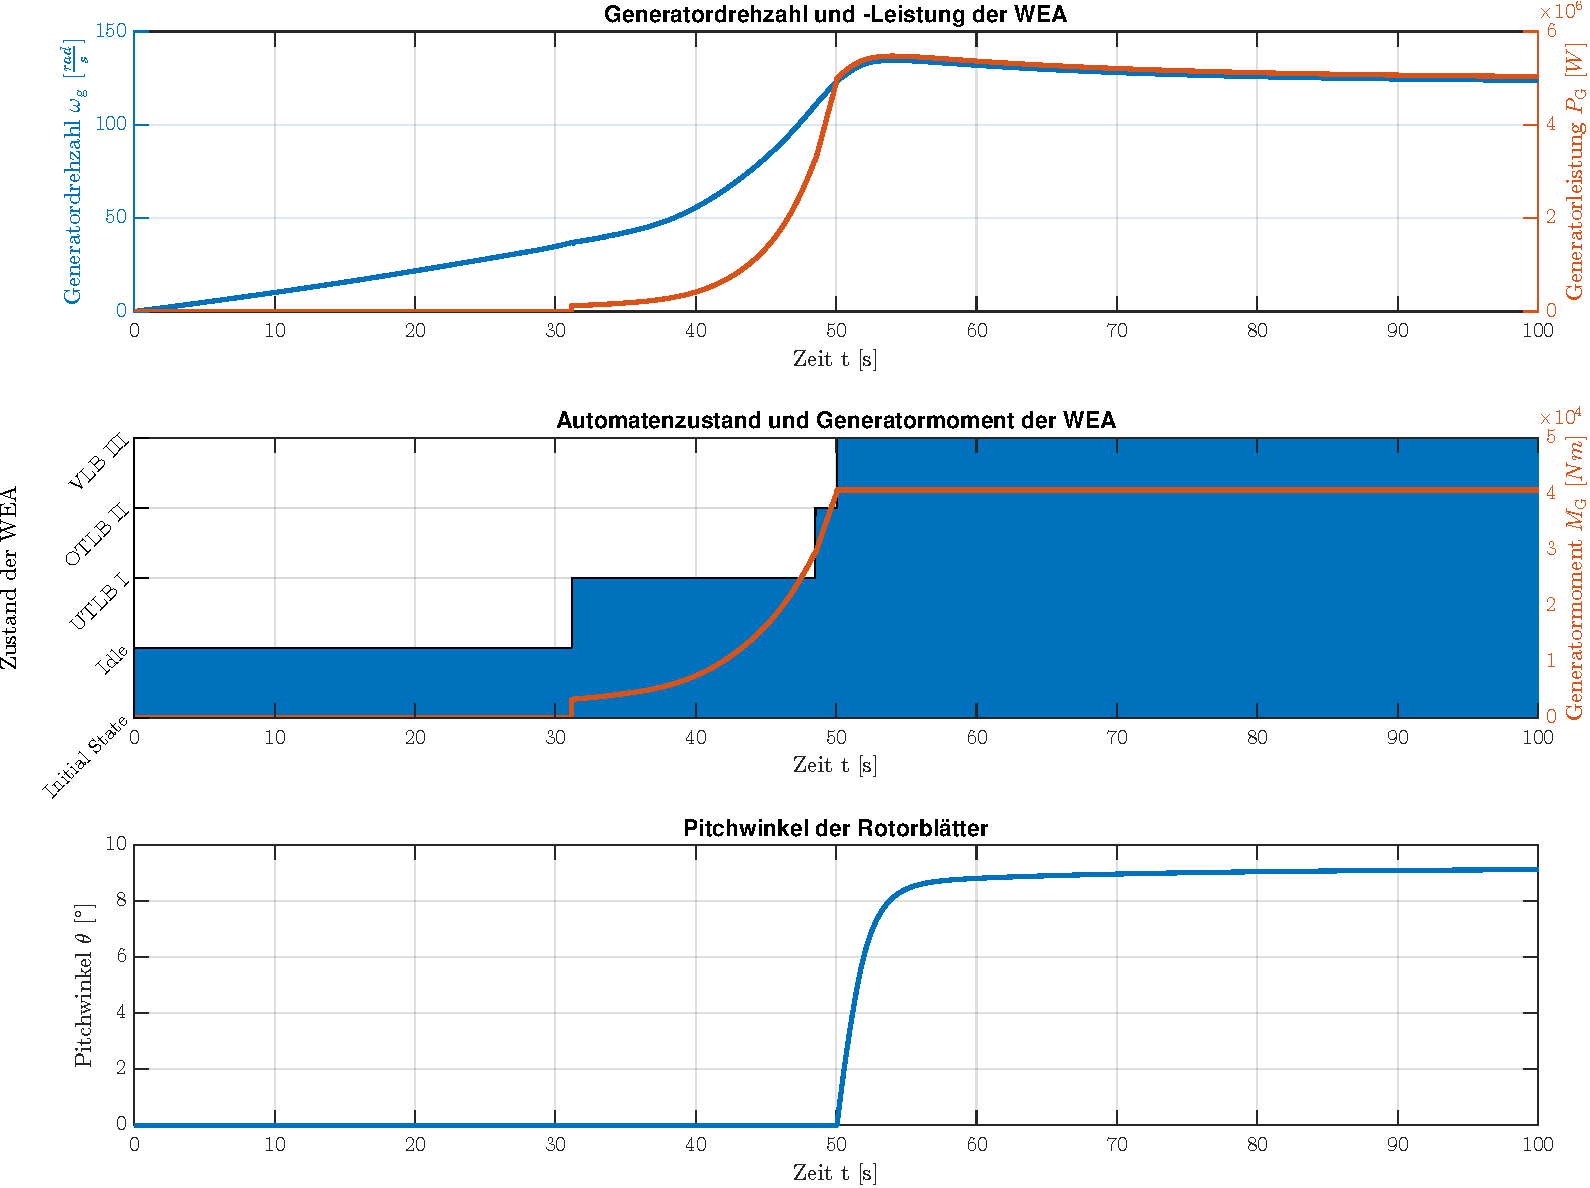
\includegraphics[width=1\textwidth]{Bilder/Kapitel 6/Reglervalidierung/const_wind_high.pdf}}
   \caption[Simulationsergebnisse schneller konstanter Wind]{Simulationsergebnisse bei einem eingeprägten konstanten Wind von $\SI{14}{\frac{m}{s}}$}
   \label{fig:Bild4.9}
\end{figure}

\autoref{fig:Bild4.10} zeigt einen Vergleich mehrerer Windgeschwindigkeiten in einem Diagramm. Dargestellt werden die Generatorwinkelgeschwindigkeit \acs{omegaG}, die Generatorleistung \acs{PG} und der Pitchwinkel \acs{theta}. Auf der linken Seite der Diagramme ist jeweils eine Legende mit den Windgeschwindigkeiten, bei welchen ein Kurvenverlauf entstanden ist.\\
Zunächst wird die Generatorwinkelgeschwindigkeit betrachtet. Es fällt auf, dass alle Kurven zwei Biegestellen besitzen. Bei der ersten vergrößert sich die Steigung und bei der zweiten sinkt sie. Je größer die eingeprägte Windgeschwindigkeit ist, desto schneller werden die beiden Stellen erreicht. 

\begin{figure}[H]
   \centering
   \fbox{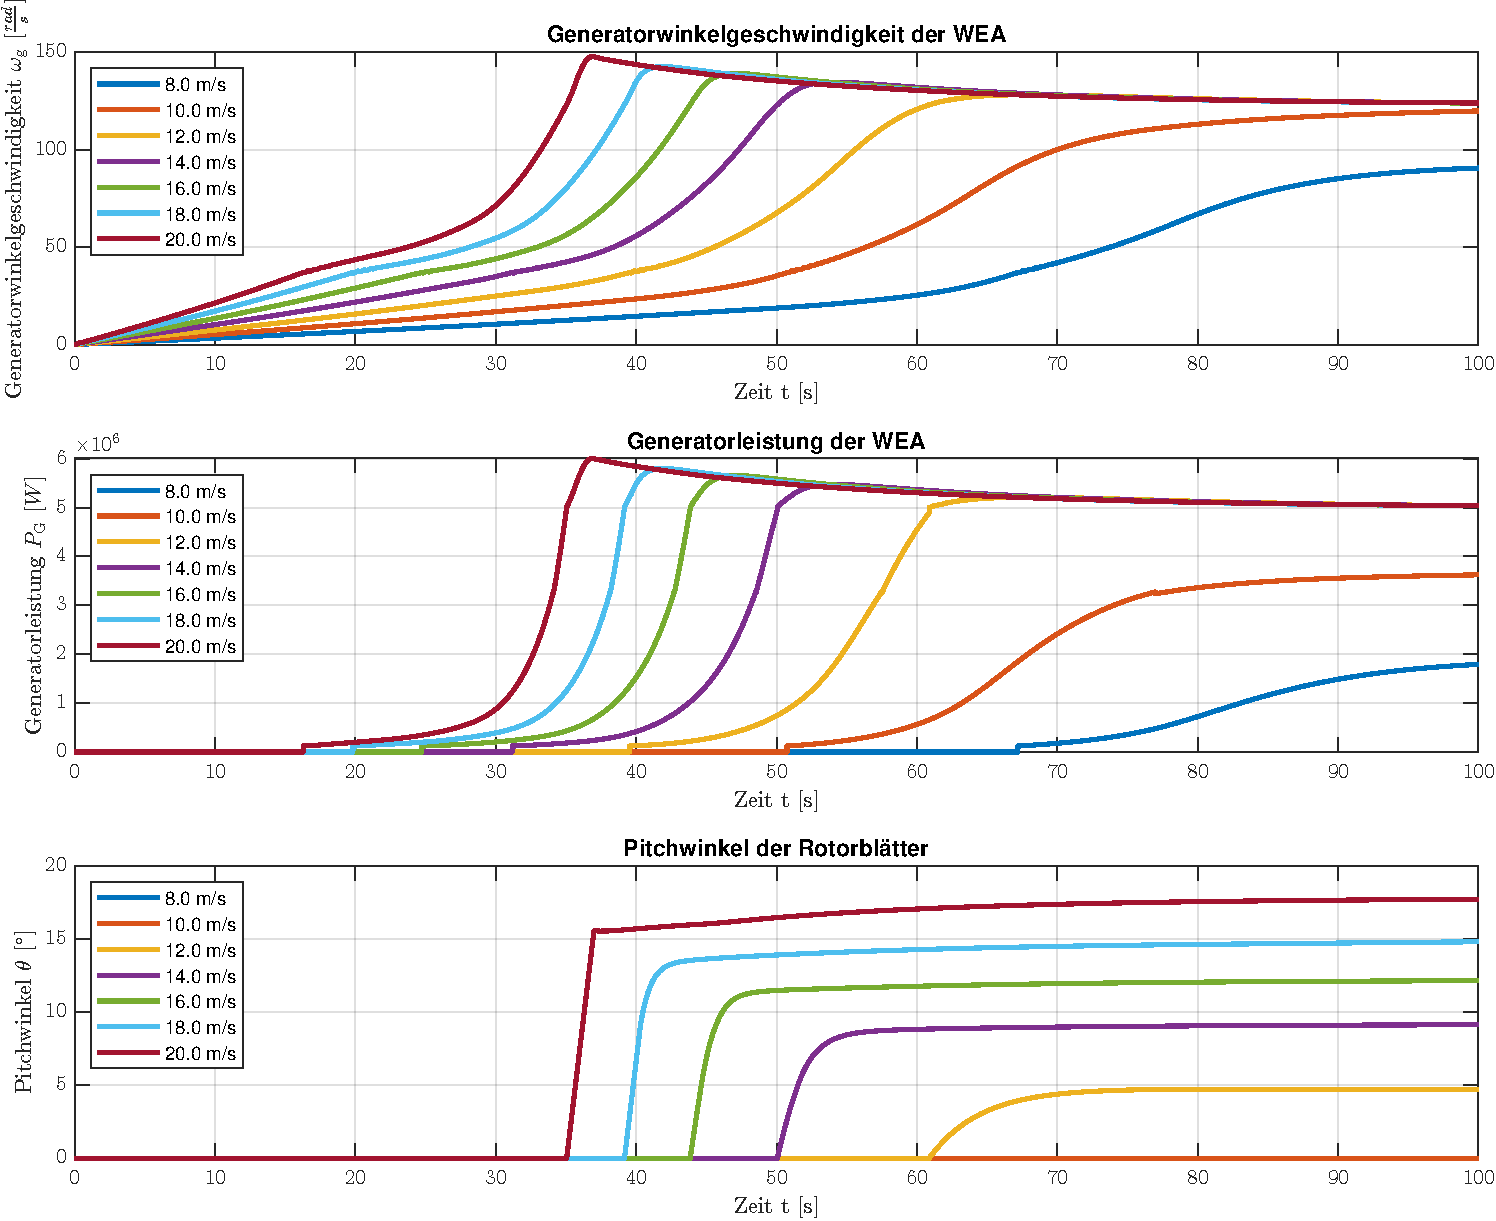
\includegraphics[width=1\textwidth]{Bilder/Kapitel 6/Reglervalidierung/const_wind_vgl.pdf}}
   \caption[Vergleich bei Verschiedenen Windgeschwindigkeiten]{Vergleich der Simulationsergebnisse bei verschiedenen konstanten Windgeschwindigkeiten zwischen $\SI{8}{\frac{m}{s}}$ bis $\SI{20}{\frac{m}{s}}$}
   \label{fig:Bild4.10}
\end{figure}

Es fällt weiterhin auf, dass bei $v_1 = \SI{8}{\frac{m}{s}}$ nicht die Nenndrehzahl als Endwert erreicht wird. Grund dafür ist, dass bei dieser recht kleinen Windgeschwindigkeit der obere Teillastbereich nicht erreicht wird und somit die Drehzahl nicht auf die Nenndrehzahl geregelt wird. Ebenfalls zu erkennen ist, dass je stärker der Wind ist, desto größer das Überschwingen der Drehzahl ist. Dies ist zu begründen über die Größe des benötigten Pitchwinkels, um die Drehzahl konstant zu halten. Umso größer der benötigte Pitchwinkel, desto größer das Überschwingen. Nach Abschluss des Ausgleichvorgangs wird jedoch für alle Windgeschwindigkeiten, die Drehzahlen für mindestens den oberen Teillastbereich erreichen, die Generatordrehzahl gleich der Nenndrehzahl.\\
Auch im mittleren Bereich der Abbildung sind gleiche Zusammenhänge für die Generatorleistung zu erkennen. Wesentlicher Unterschied zu der Drehzahldarstellung ist, dass erst ab dem Erreichen des unteren Teillastbereiches eine Leistung ausgegeben wird. Der Zeitpunkt dafür wird bei steigender Windgeschwindigkeit immer früher erreicht. Die Nennleistung kann bei allen Winden bis auf $v_1 = \SI{8}{\frac{m}{s}}$ und $v_1 = \SI{10}{\frac{m}{s}}$ hergestellt werden. Die beiden erwähnten Windgeschwindigkeiten reichen nicht aus, um eine ausreichend große Drehzahl für den Volllastbereich zu generieren. Erst im Volllastbereich wird auf die Nennleistung geregelt.\\
Im untersten Abschnitt der Grafik wird der Pitchwinkel gezeigt. Da das Pitchen erst ab dem Volllastbereich einsetzt, bleiben die Pitchwinkel für $v_1 = \SI{8}{\frac{m}{s}}$ und $v_1 = \SI{10}{\frac{m}{s}}$ dauerhaft bei $0^\circ$. Das Eintreten des Volllastbereiches bestimmt den Zeitpunkt des Pitch-Beginns. Mit steigender Windgeschwindigkeit verringert sich die Zeit bis zum Beginn der Pitch-Regelung.\\

% ---------------------------------

Als nächster Windtyp werden Windböen getestet. Es tritt genau eine Böe bei einer ansonsten konstanten Windgeschwindigkeit auf. Es soll gezeigt werden, welchen Einfluss eine einzelne starke Änderung des Windes auf die Regelung hat. Es werden an dieser Stelle zwei unterschiedlich große Böen auf das Modell eingeprägt.\\
\autoref{fig:Bild4.11} zeigt zunächst die Simulationsergebnisse für einen Wind mit $v_1 = \SI{8}{\frac{m}{s}}$ mit einer Böenamplitude von \ca $\SI{11.5}{\frac{m}{s}}$. Im Vergleich zu \autoref{fig:Bild4.7} sind kaum Unterschiede zu erkennen, was als positiv zu bewerten ist. Lediglich der Zeitpunkt des Eintritts des unteren Teillastbereiches wird um ein bis zwei Sekunden verringert und die Endwerte für Generatorleistung, -winkelgeschwindigkeit und -moment werden minimal größer.

\begin{figure}[H]
   \centering
   \fbox{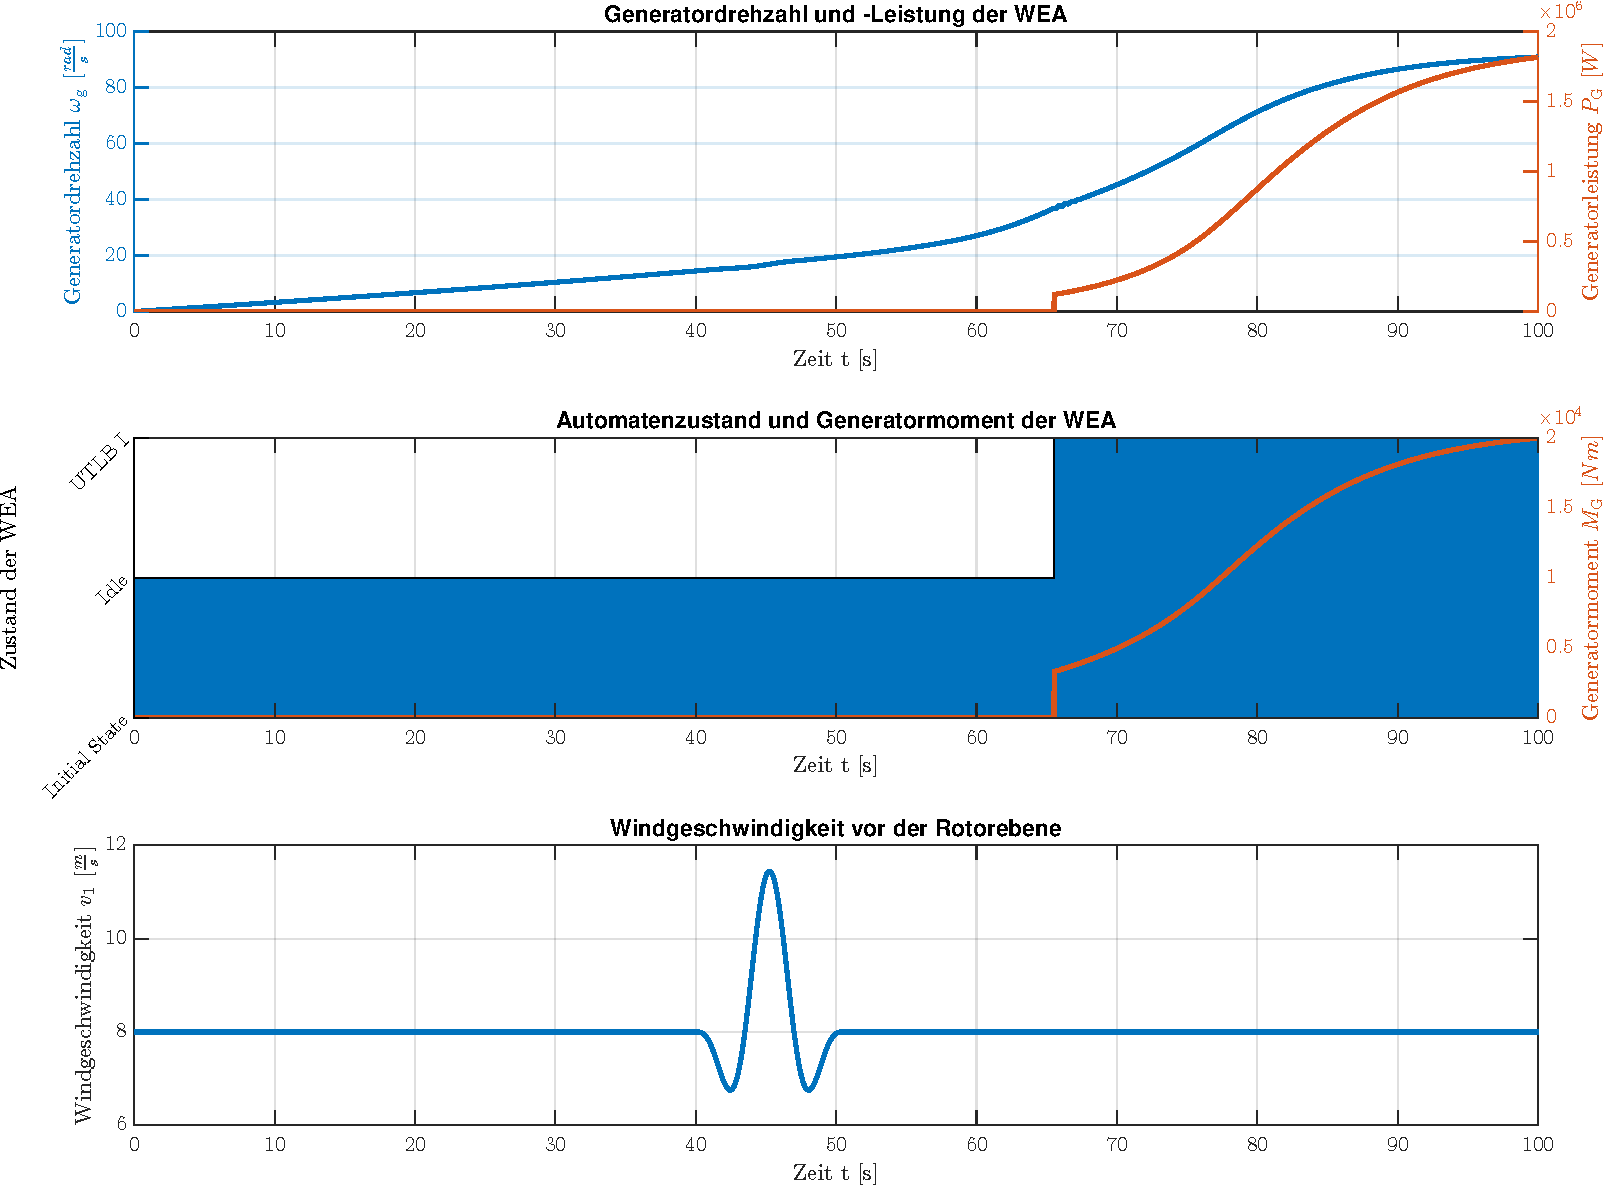
\includegraphics[width=1\textwidth]{Bilder/Kapitel 6/Reglervalidierung/gust_low.pdf}}
   \caption[Windböensimulation bei langsamem Wind]{Simulationsergebnisse für einen konstanten Wind mit $v_1 = \SI{8}{\frac{m}{s}}$ und einer Windböe mit einer Amplitude bei $\SI{11.5}{\frac{m}{s}}$}
   \label{fig:Bild4.11}
\end{figure}

Bei \autoref{fig:Bild4.12} ist im Gegensatz zur vorangegangenen Grafik kein Unterschied in den stationären Endwerten im Vergleich zu \autoref{fig:Bild4.9} zu erkennen. Zu begründen ist dies durch den Regler des Volllastbereiches, der zum Ziel hat, das Moment und die Drehzahl konstant zu halten. Da das Auftreten der Böe im unteren und oberen Teillastbereich stattfindet, werden jedoch sowohl die Drehzahl, als auch das Moment und die Leistung beeinflusst. Durch den lokalen Anstieg der Windgeschwindigkeit beschleunigt der Rotor leicht, was zu einer Vergrößerung der Generatordrehzahl führt. Da die Drehzahl steigt, sinkt die Steigung des Momentes und der dazu proportionalen Leistung kurzzeitig ab.

\begin{figure}[H]
   \centering
   \fbox{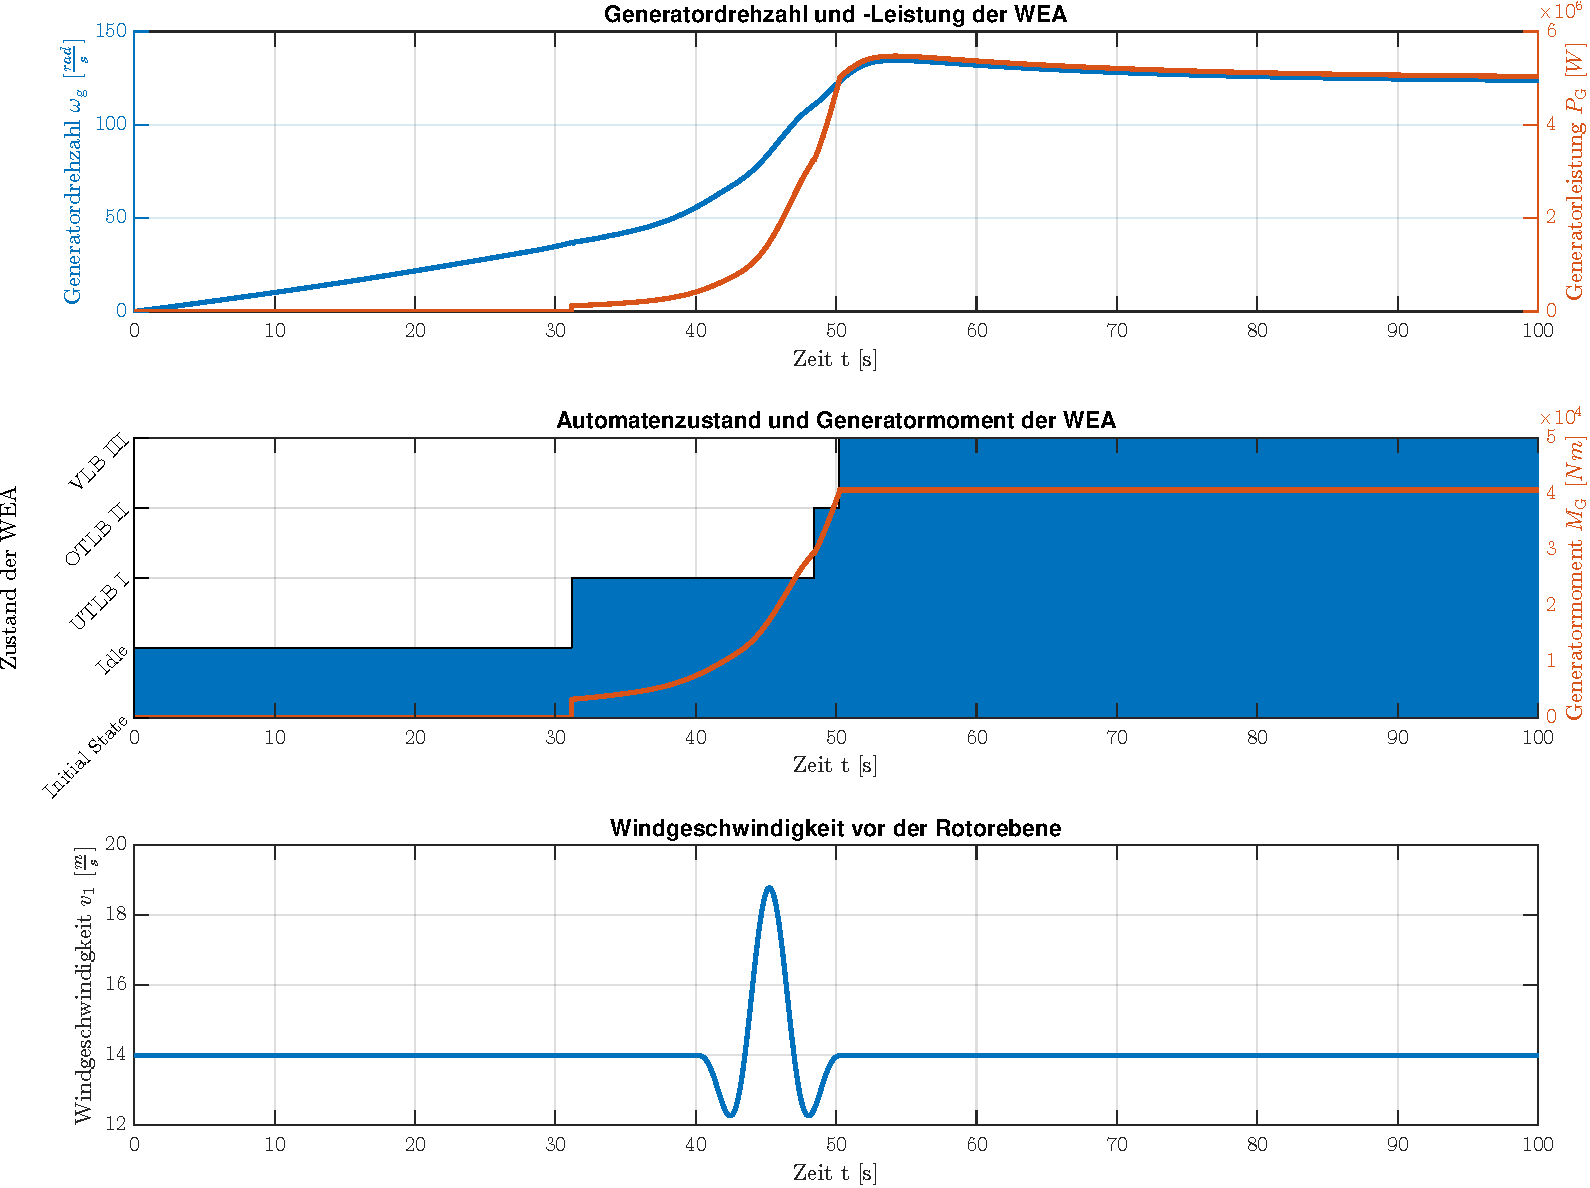
\includegraphics[width=1\textwidth]{Bilder/Kapitel 6/Reglervalidierung/gust_high.pdf}}
   \caption[Windböensimulation bei schnellem Wind]{Simulationsergebnisse für einen konstanten Wind mit $v_1 = \SI{14}{\frac{m}{s}}$ und einer Windböe mit einer Amplitude bei $\SI{19}{\frac{m}{s}}$}
   \label{fig:Bild4.12}
\end{figure}

% ---------------------------------

Im Folgenden soll das WEA-Modell inklusive der Regelstruktur gegen turbulente Winde getestet werden. Die getesteten Windreihen kommen realen Winden sehr nah. Somit kann über die Bewertung der nachfolgenden drei Abbildungen eine Aussage über die Anwendbarkeit der entworfenen Regler in der Realität getroffen werden. Interessant bei der Untersuchung ist vor allem das Verhalten bei dem Überschreiten der kritischen Windgeschwindigkeit \acs{vkrit}. Ebenfalls validiert werden soll die Fähigkeit des Pitchreglers, das Generatormoment und die Generatordrehzahl im Volllastbereich möglichst konstant zu halten.\\
\autoref{fig:Bild4.13} zeigt die Simulationsergebnisse bei einer Belastung des Modells mit einem turbulenten Wind mit $v_1 = \SI{8}{\frac{m}{s}}$ im Mittel. Im Vergleich zu der Abbildung bei konstantem Wind (\autoref{fig:Bild4.7}) fallen nur im hinteren Bereich ab \ca $\SI{85}{s}$ signifikante Unterschiede in den Kurvenverläufen auf. Zunächst beschleunigt der Antriebsstrang, bis die maximale Drehzahl und das maximale Drehmoment bei gegebenem Wind erreicht sind. Durch die turbulenten Schwankungen im Wind und der Leistungsoptimierung im unteren Teillastbereich (\vgl \autoref{tab:Tabelle4.1}) schwanken die Drehzahl, das Moment und die Leistung des Rotors proportional zum Wind mit. 

\begin{figure}[H]
   \centering
   \fbox{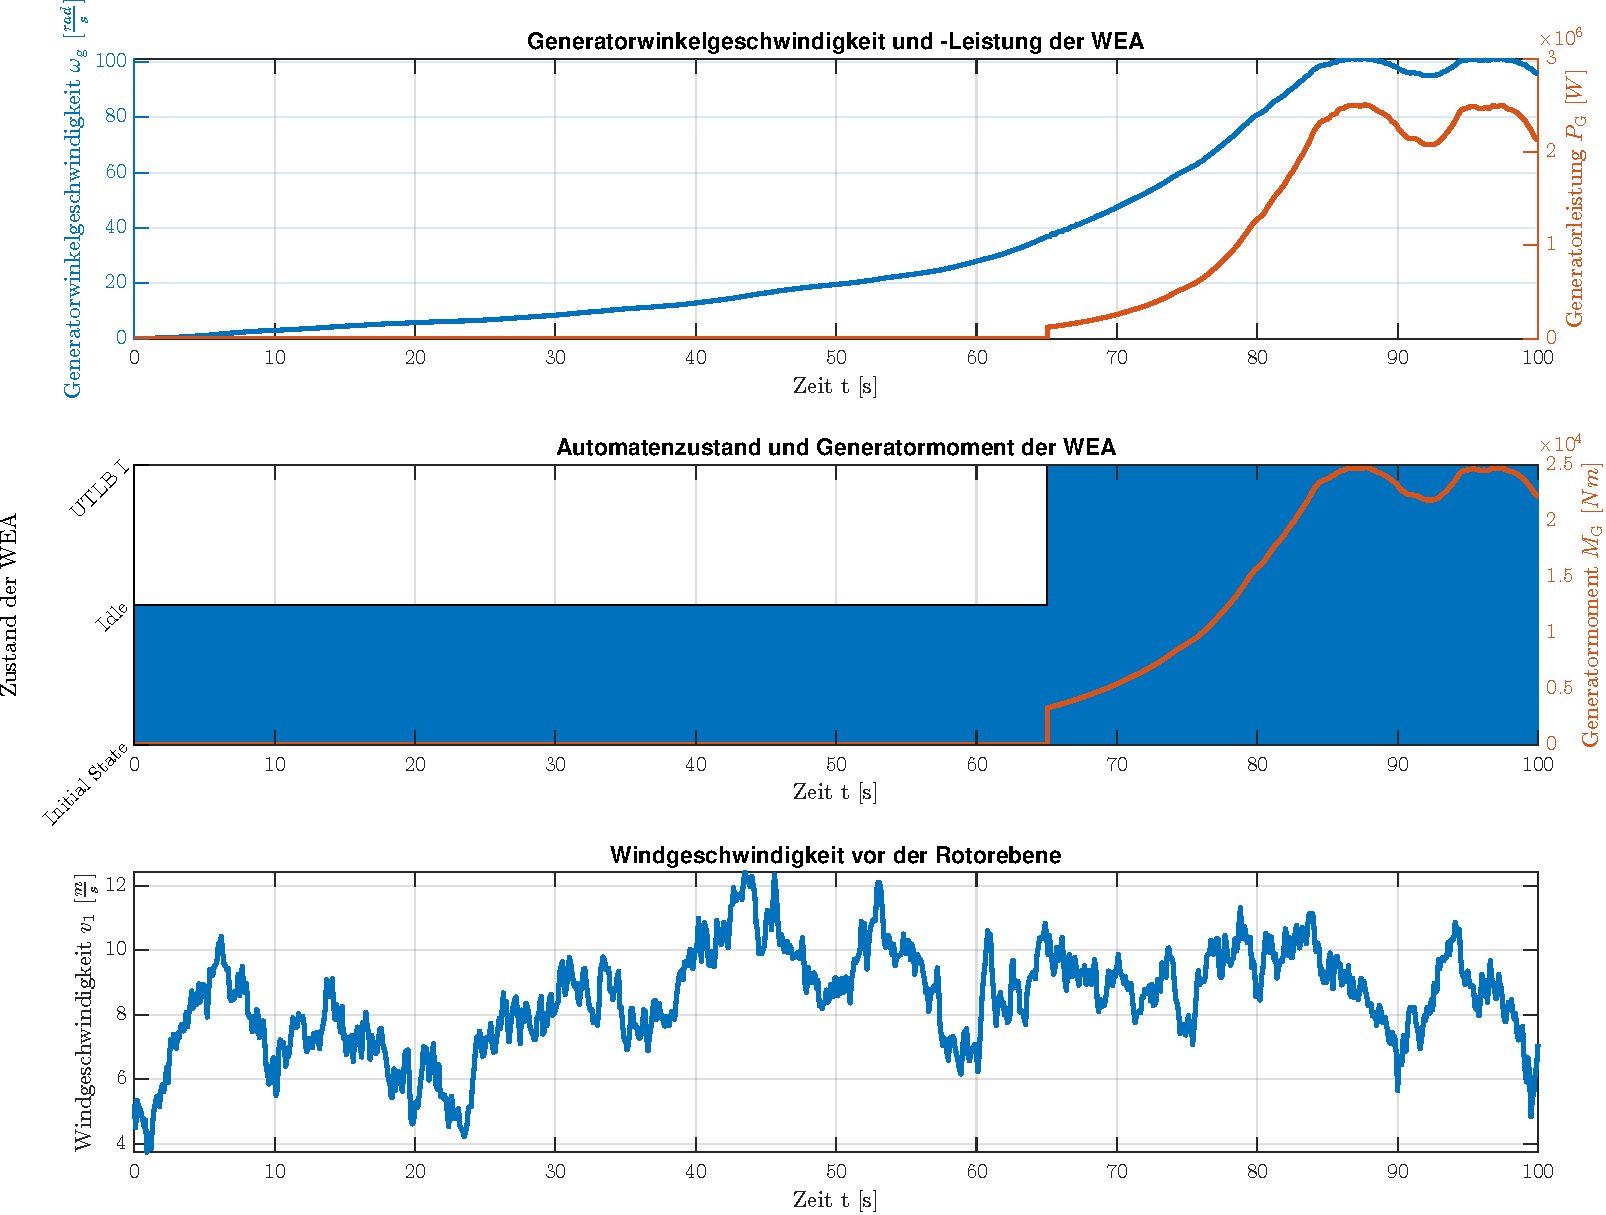
\includegraphics[width=1\textwidth]{Bilder/Kapitel 6/Reglervalidierung/turb_low.pdf}}
   \caption[Simulationsergebnisse bei langsamen turbulenten Winden]{Simulationsergebnisse bei turbulenten Winden mit einer mittleren Windgeschwindigkeit von $\SI{8}{\frac{m}{s}}$}
   \label{fig:Bild4.13}
\end{figure}

In \autoref{fig:Bild4.14} ist ein ausreichend starker Wind dargestellt, so dass der Vollastbereich der Anlage erreicht wird. Gut zu erkennen ist im oberen Bereich der Abbildung, dass nach Abklingen des Überschwingens im Vollastbereich die Leistung und die Drehzahl annähernd konstant im Nennwert gehalten werden. Somit ist festzustellen, dass die Regelung des Pitchwinkels funktional ist. Besonders gut ist dies im untersten Teil der Grafik zu erkennen. Es fällt auf, dass der Pitchwinkel proportional zur Windgeschwindigkeit Änderungen erfährt. Lediglich ein kleines Delay ist auszumachen, welches aufgrund der Stellgrößenbegrenzung des Pitchmotors auf maximal $8^\circ$/s auftritt. Ebenfalls Grund dafür ist ein leicht dämpfendes Verhalten des Pitchreglers, welches aus der Berechnung der Reglerkoeffizienten hervorgeht. Genau diese Eigenschaften sorgen dafür, dass die Generatorleistung und die Generatordrehzahl nicht exakt auf dem Nennwert verweilen.

\begin{figure}[H]
   \centering
   \fbox{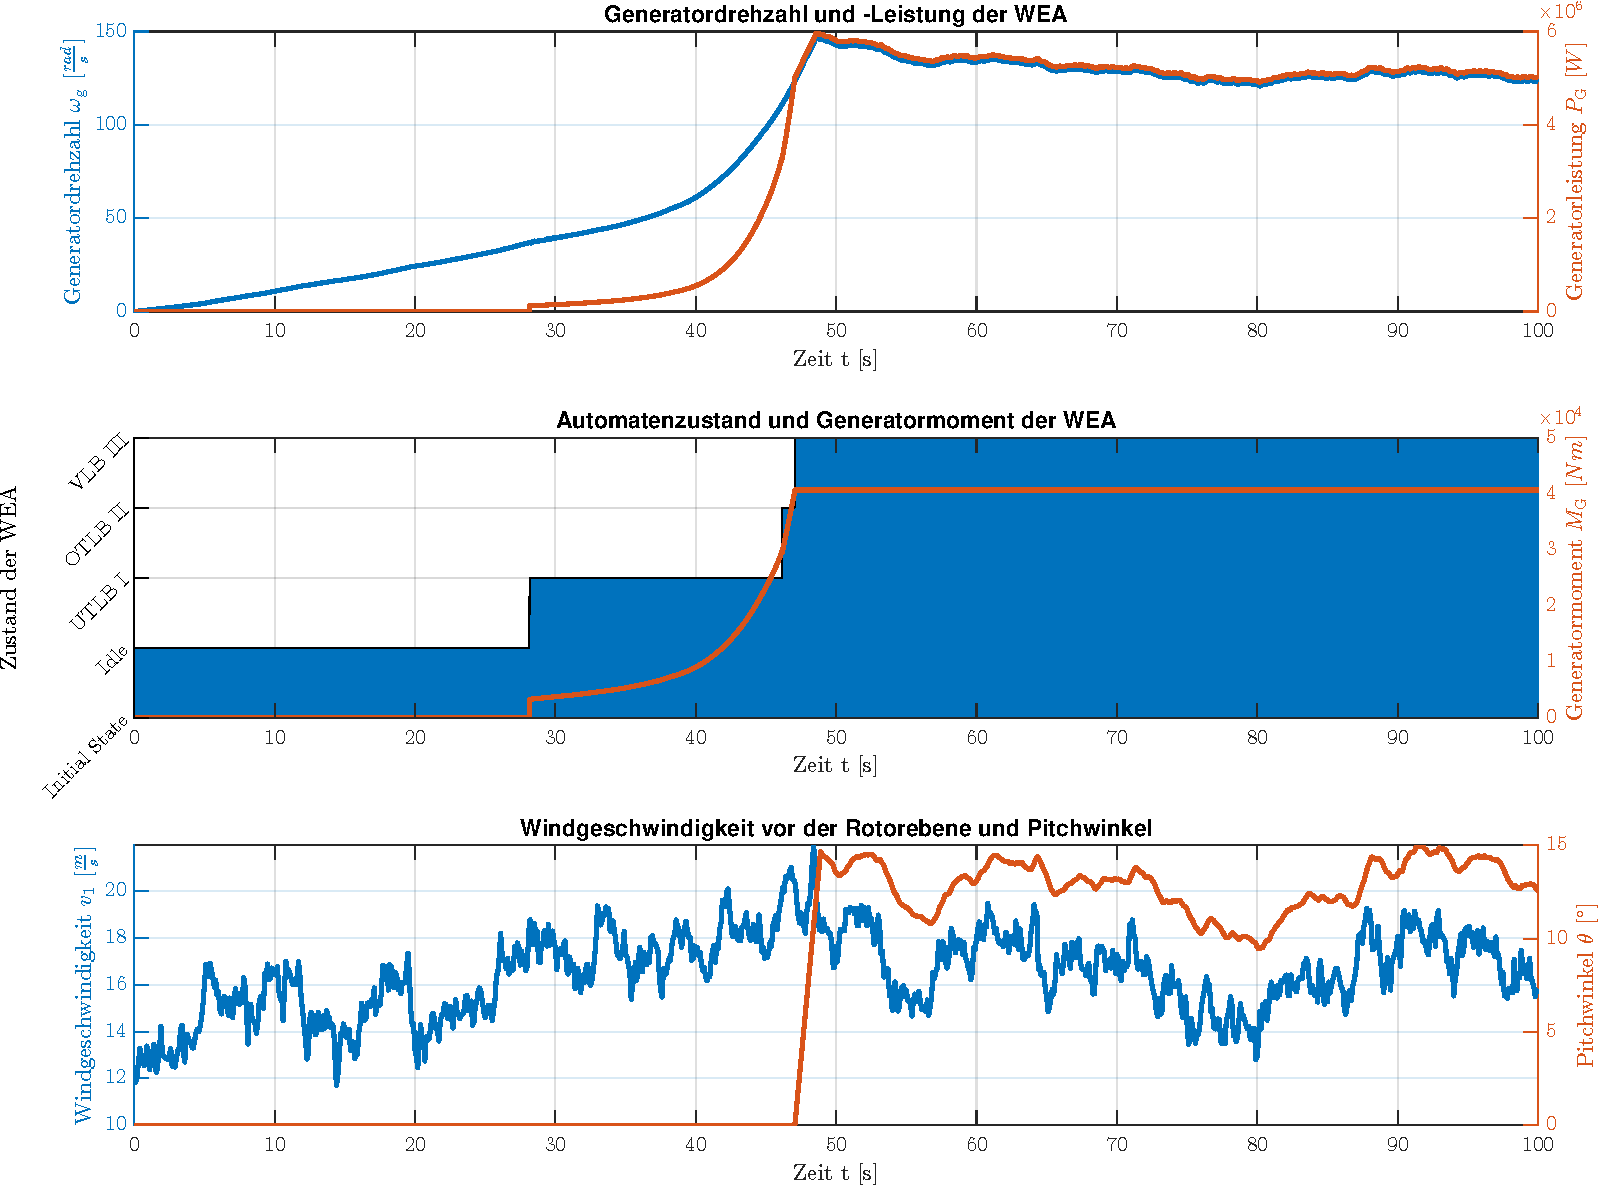
\includegraphics[width=1\textwidth]{Bilder/Kapitel 6/Reglervalidierung/turb_medium.pdf}}
   \caption[Simulationsergebnisse bei moderaten turbulenten Winden]{Simulationsergebnisse bei turbulenten Winden mit einer mittleren Windgeschwindigkeit von $\SI{16}{\frac{m}{s}}$}
   \label{fig:Bild4.14}
\end{figure}

Bei \autoref{fig:Bild4.15} soll das Verhalten der Anlage bei turbulenten Winden geprüft werden, welche die kritische Windgeschwindigkeit $\acs{vkrit} = \SI{25}{\frac{m}{s}}$ überschreiten. Die Kurvenverläufe in den ersten $\SI{75}{s}$ verhalten sich analog zu denen in \autoref{fig:Bild4.14}. Anschließend wird mehrmals kurzzeitig die maximale Schwelle überschritten, was gut am Verlauf des Windes im unteren Bereich von \autoref{fig:Bild4.15} zu sehen ist. Im mittleren Teil der Grafik ist zu erkennen, dass die Anlage in den E-Stop-Zustand (Nothalt) umschaltet. Erst nach unterschreiten von $90\%$ der kritischen Windgeschwindigkeit (\vgl \autoref{fig:Abbildung4.6} Zustand E-Stop) geht die WEA wieder zurück in den Idle-Zustand und läuft nachfolgend wieder an. Da der Wind im Fall der gezeigten Simulationsergebnisse nach kurzer Zeit wieder die kritische Windgeschwindigkeit überschreitet, geht die Anlage erneut in den Stop-Zustand. Das schnelle Wechseln der Zustände ist möglicherweise als nicht optimal anzusehen und bedarf einer Optimierung. Einen Vorschlag dafür liefert der \autoref{ausblick} \texttt{Ausblick}.  

\begin{figure}[H]
   \centering
   \fbox{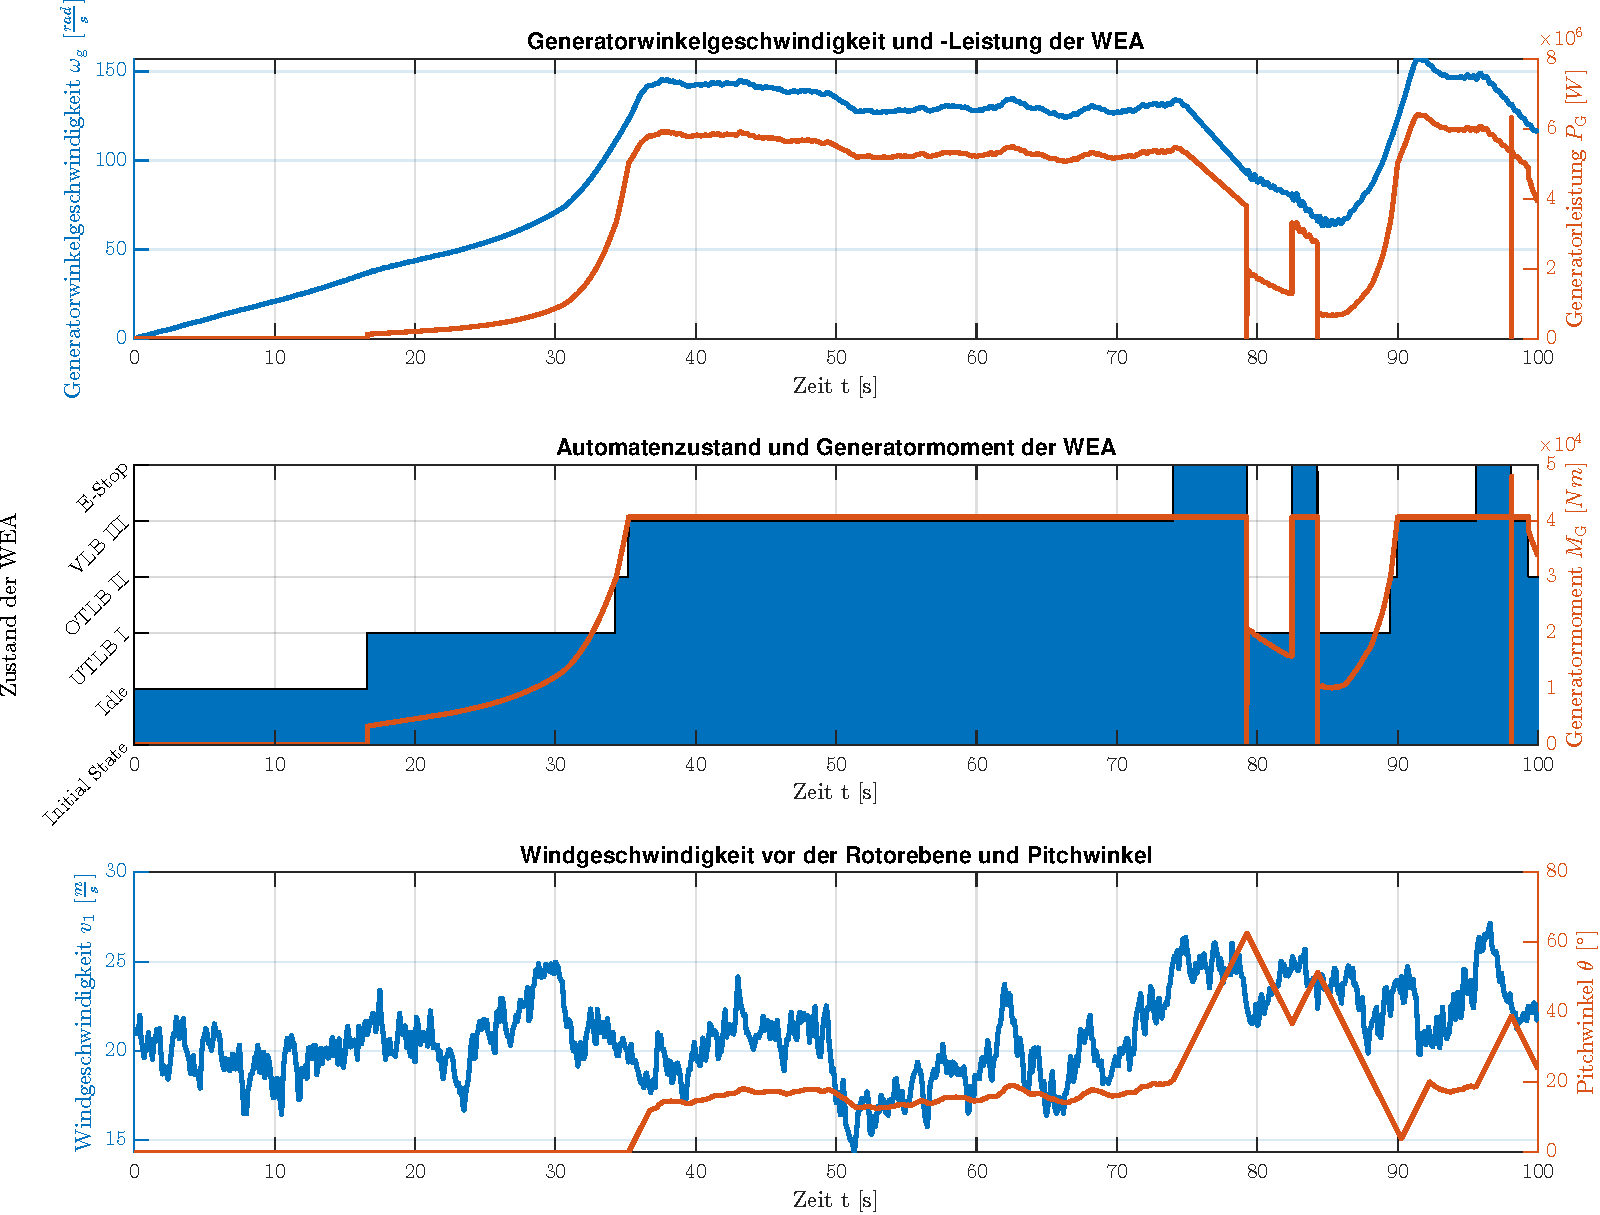
\includegraphics[width=1\textwidth]{Bilder/Kapitel 6/Reglervalidierung/turb_high.pdf}}
   \caption[Simulationsergebnisse bei schnellen turbulenten Winden]{Simulationsergebnisse bei turbulenten Winden mit einer mittleren Windgeschwindigkeit von $\SI{20}{\frac{m}{s}}$}
   \label{fig:Bild4.15}
\end{figure}

% ---------------------------------

Zuletzt wird eine Analyse der Ergebnisse der Simulation von Modell und Reglern gegen einen stufenförmigen Wind vorgenommen. Ziel ist es insbesondere das transiente Verhalten der Regler zu untersuchen, welches als besonders kritisch bei der maximalen Belastung des Modells durch unendlich steile Flanken im Wind einzustufen sind. Weiterhin ist der Wind in seiner letzten Stufe so gewählt, dass die Anlage bei maximaler Auslastung durch einen Wind von $v_1 = \SI{25}{\frac{m}{s}}$ betrieben wird.\\
\autoref{fig:Bild4.16} zeigt die Ergebnisse der Simulation. Beim der Betrachtung des obersten und untersten Bildausschnitts ist klar zu erkennen, dass der Sprung auf die maximale Windgeschwindigkeit für eine ruckartige Erhöhung der Beschleunigung des Rotors sorgt, was gut an der Generatorwinkelgeschwindigkeit auszumachen ist. Da die Windgeschwindigkeit und die Rotordrehzahl zu Beginn des Volllastbereiches sehr groß sind, kommt es auf Grund des initialen Pitchwinkels von $0^\circ$ zu einer starken Vergrößerung der \ac{FS}. Diese wiederum sorgt für eine Überhöhung der Generatorleistung über den Nennwert hinaus. Somit steigt der Pitchwinkel mit seiner maximalen Winkelgeschwindigkeit an, bis der benötigte Winkel erreicht ist. Da die Schubkraft durch die Vergrößerung des Pitchwinkels schnell wieder abfällt und somit auch die Leistung wieder zurückfällt, nimmt auch der Pitchwinkel wieder ab, bis sich alle Kurven zum Ende der Abbildung in einen stationären Endwert einfinden.

\begin{figure}[H]
   \centering
   \fbox{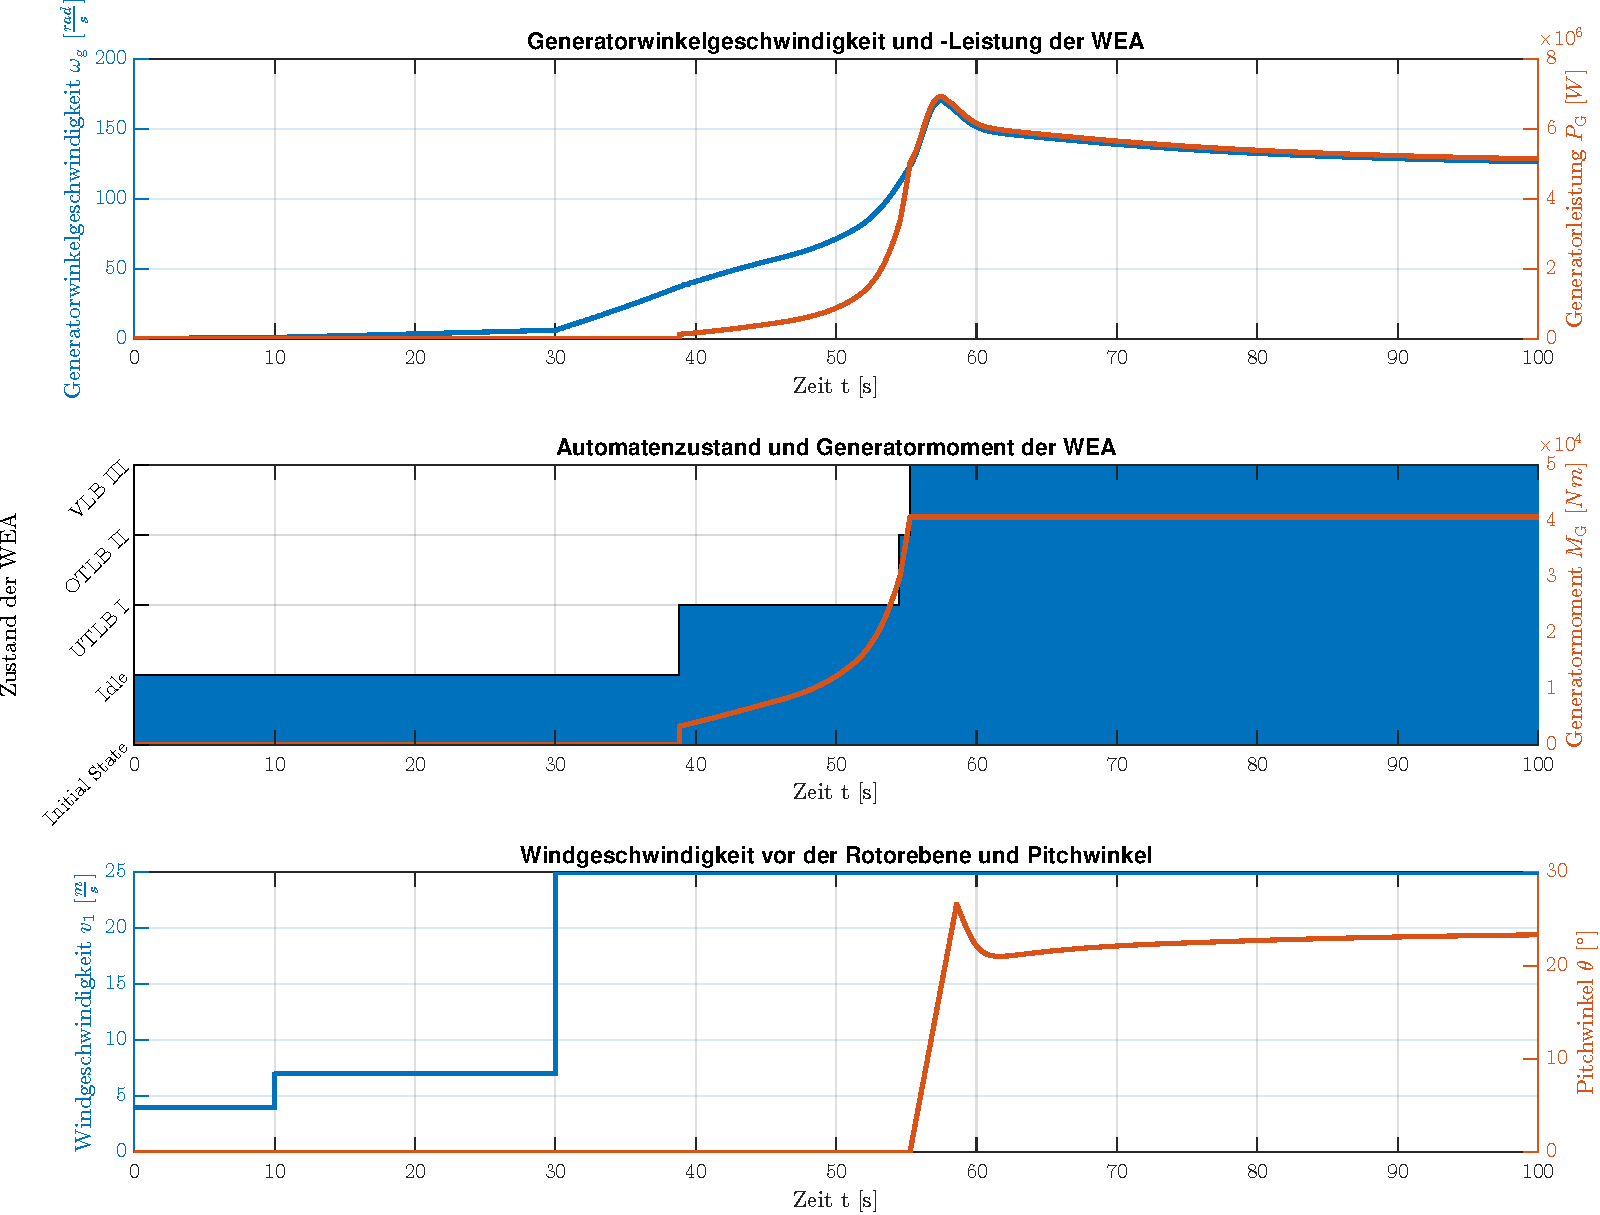
\includegraphics[width=1\textwidth]{Bilder/Kapitel 6/Reglervalidierung/wind_steps.pdf}}
   \caption[Simulationsergebnisse bei stufenförmigem Wind]{Simulationsergebnisse für einen eingeprägten stufenförmigem Wind bei einer maximalen Windgeschwindigkeit von $\SI{25}{\frac{m}{s}}$}
   \label{fig:Bild4.16}
\end{figure}

\subsubsection{Validierung der Regelziele}

Wie bereits in \autoref{regelziel} postuliert wurde, ist die Regelung in drei Arbeitsbereiche eingeteilt worden. Im unteren und oberen Teillastbereich findet eine Leistungsoptimierung statt. Im Vollastbereich wird hingegen die Leistung begrenzt. Besagte Regelziele sollen an \autoref{fig:Bild4.17} und \autoref{fig:Bild4.18} aufgezeigt werden.\\

\begin{figure}[H]
   \centering
   \fbox{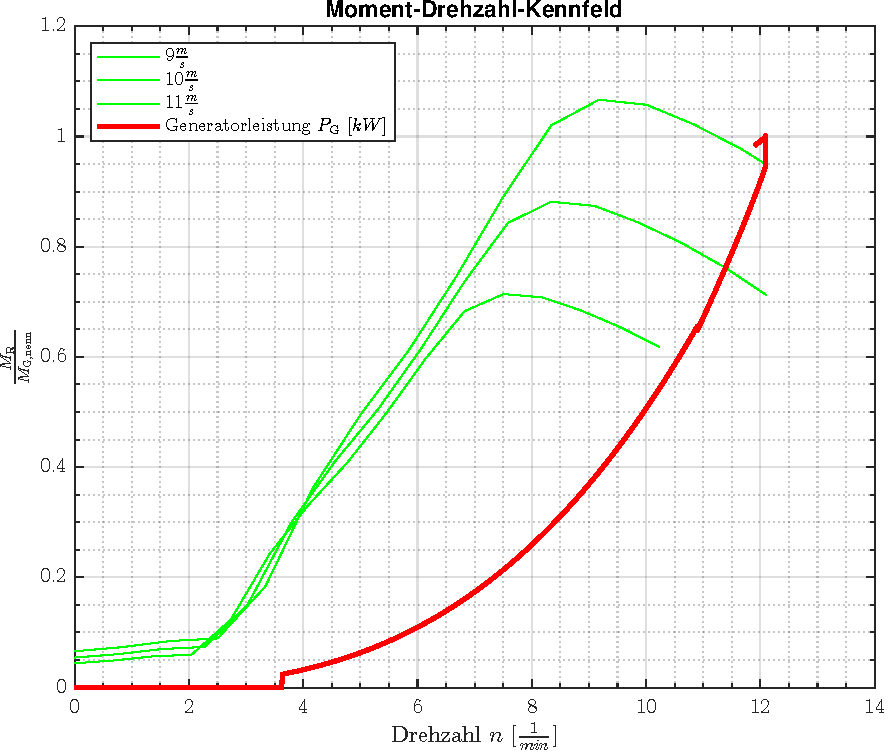
\includegraphics[width=0.95\textwidth]{Bilder/Kapitel 6/Reglervalidierung/moment_drehzahl_kennfeld.pdf}}
   \caption[Simulation des Moment-Drehzahl-Kennfelds]{Simulationsergebnisse für die Darstellung des Moment-Drehzahl-Kennfelds}
   \label{fig:Bild4.17}
\end{figure}
Zunächst wird der untere Teillastbereich betrachtet. Ziel war es die Drehzahl optimal an die Windgeschwindigkeit anzupassen, so dass sich ein optimales Anströmverhältnis ergibt. Das heißt, dass mit ansteigender Windgeschwindigkeit \acs{v1} stets das Leistungsmaximum aus der jeweiligen Windleistung entnommen wird (also $c_{\mathrm{P}} = c_{\mathrm{P,max}}$). \autoref{fig:Bild4.17} zeigt genau diesen Zusammenhang an der Kurve der Generatorleistung \acs{PG}. Wird die minimale Drehzahl ($30\%$ der Nenndrehzahl) überschritten, steigt das Rotormoment mit steigender Drehzahl.\\
Gut zu erkennen ist, dass ab $95\%$ der Nennleistung die Nenndrehzahl erreicht ist. Nun befindet sich die WEA im oberen Teillastbereich und lediglich das Drehmoment kann bis zum Nennmoment ansteigen. Der Bereich des oberen Teillastbereiches ist gut an dem senkrechten Verlauf der Generatorleistung zu erkennen.\\

\begin{figure}[H]
   \centering
   \fbox{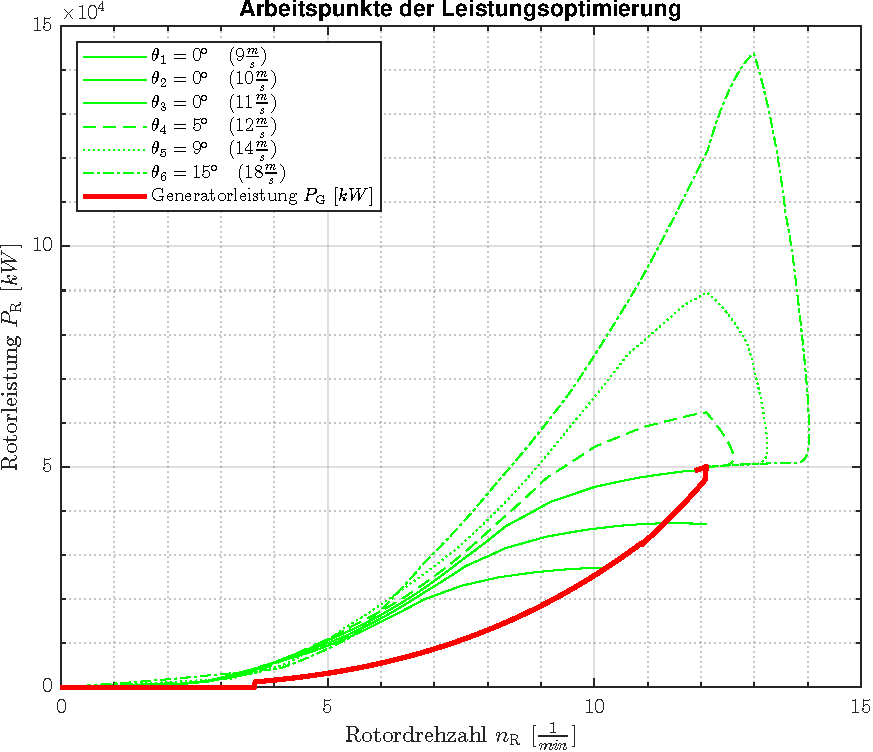
\includegraphics[width=0.95\textwidth]{Bilder/Kapitel 6/Reglervalidierung/valid_arbeitspunkte.pdf}}
   \caption[Simulation der Leistungsoptimierung]{Simulationsergebnisse für die Leistungsoptimierung zur Darstellung der Arbeitspunkte des Systems}
   \label{fig:Bild4.18}
\end{figure}

Ist das Nennmoment erreicht, bleiben sowohl Drehzahl als auch Moment konstant auf den Nennwerten. Der sich anschließende Bereich ist der Volllastbereich. Aus \autoref{fig:Bild4.18} geht hervor, dass bei größeren Winden nach erreichen der Nennwerte ein Pitchwinkel $>0^\circ$ eingestellt wird. Der Pitchwinkel steigt mit steigender Windgeschwindigkeit. Folglich wird die Leistung begrenzt.\\
Ebenfalls aus \autoref{fig:Bild4.18} abzulesen sind die Arbeitspunkte der Leistungsoptimierung. Es können die Verläufe aus \autoref{kennfelder} nachgebildet werden. Insbesondere \autoref{fig:Bild2.13} wird durch die Simulationsergebnisse bestätigt.

\subsubsection{Prüfung der Einhaltung der Constraints}

Ziel dieses Abschnittes ist zu Prüfen, inwiefern die gegebenen Begrenzungen des Systems in der Simulation eingehalten werden. Verifiziert werden muss insbesondere, inwieweit die Generatorleistung den geforderten Nennwert überschreitet, und ob es zu großen Auslenkungen der Rotorblätter und des Turmes kommt.\\
Begonnen wird zunächst mit der Validierung der Regler am Antriebsstrangmodell, welches in \autoref{modellierung_antriebsstrang} beschrieben ist. Zu erwarten ist, dass insbesondere hohe Windgeschwindigkeiten kritisch für die Einhaltung der Constraints sind.

\begin{figure}[H]
   \centering
   \fbox{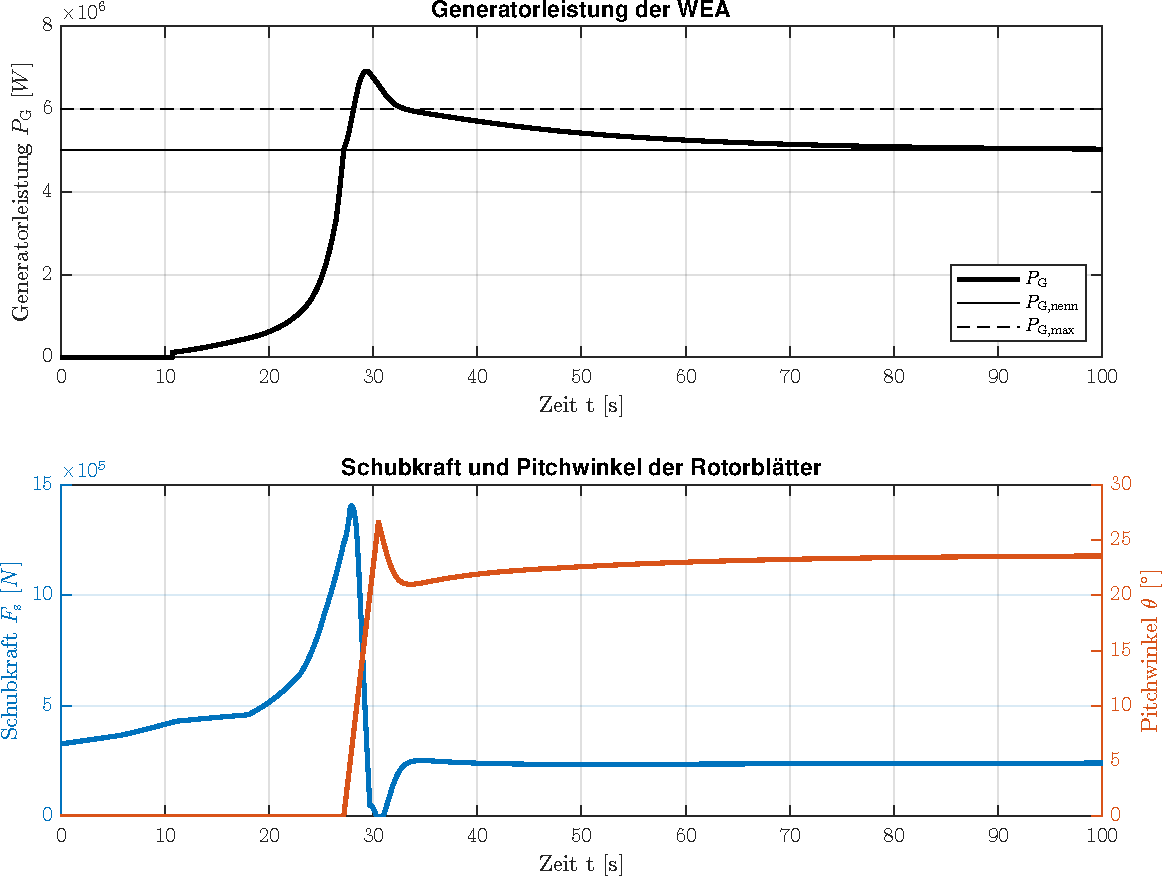
\includegraphics[width=0.85\textwidth]{Bilder/Kapitel 6/Reglervalidierung/constraint_leistung.pdf}}
   \caption[Constraint Leistungsbegrenzung]{Validierung der Leistungsbegrenzung bei $v_1 = \SI{25}{\frac{m}{s}}$}
   \label{fig:Bild4.19}
\end{figure}

\autoref{fig:Bild4.19} zeigt die Simulationsergebnisse zur Prüfung der Leistungsbegrenzung auf maximal 1.2-fache Nennleistung. Es kann festgehalten werden, dass bei sehr großen Windgeschwindigkeiten der Nennwert mehr als $20\%$ überschritten wird. Grund dafür zeigt sich in der unteren Hälfte der Grafik. Insbesondere im endenden unteren Teillastbereich und Volllastbereich steigt die Schubkraft stark an. Der Pitchvorgang beginnt jedoch erst mit $\acs{theta} = 0^\circ$ im Volllastbereich. Somit steigt die Rotordrehzahl weit über die Nenndrahzahl an, was wiederum auch zu einer übermäßig großen Steigerung der Leistung führt.\\

Weiterhin soll die implementierte Regelung und das Gesamtmodell für besonders kritische Winde auf die auftretenden Turm- und Blattauslenkungen untersucht werden. Die Eigenschaften dieses Teilmodells sind in \autoref{turm_blatt} beschrieben.\\

\begin{figure}[H]
   \centering
   \fbox{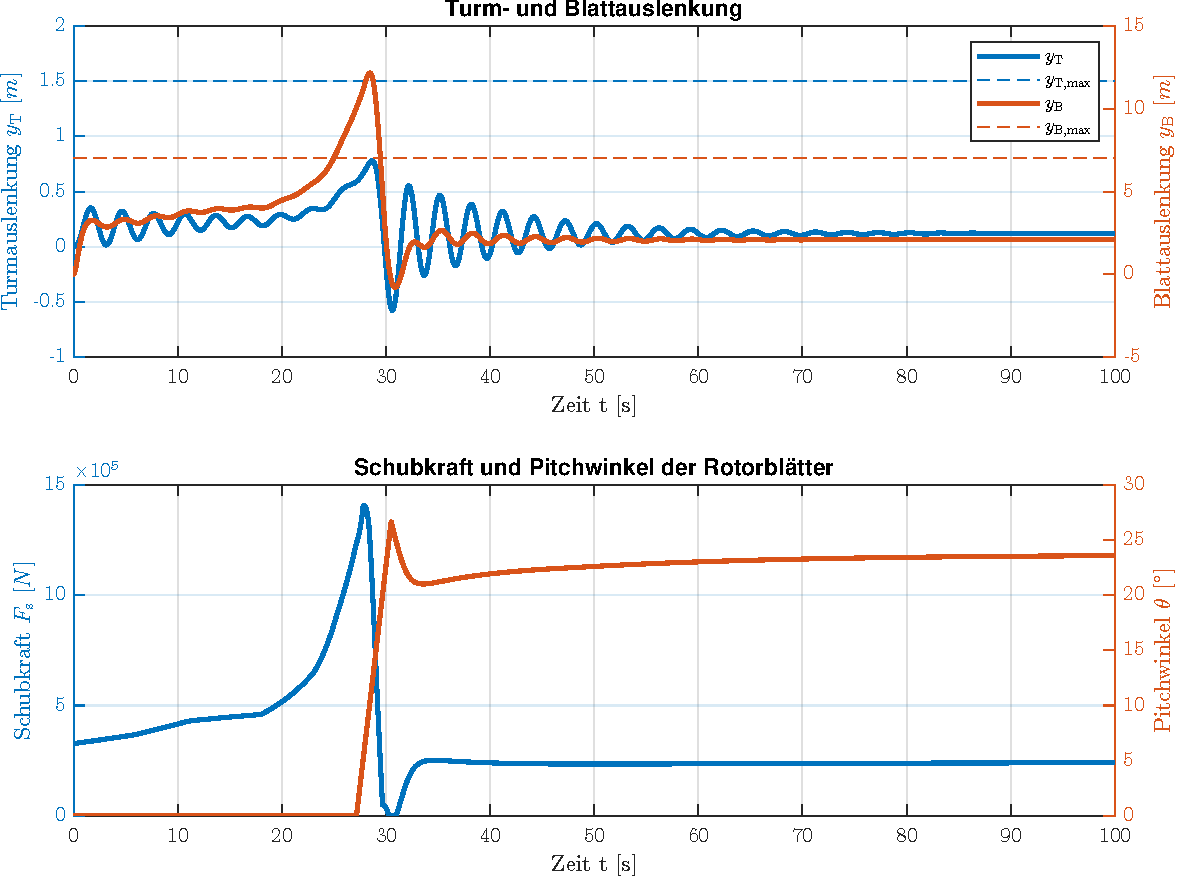
\includegraphics[width=1\textwidth]{Bilder/Kapitel 6/Reglervalidierung/constraint_auslenkung.pdf}}
   \caption[Constraint Turm- und Blattauslenkung]{Validierung der Turm- und Blattauslenkungen bei $v_1 = \SI{25}{\frac{m}{s}}$}
   \label{fig:Bild4.20}
\end{figure}

\autoref{fig:Bild4.20} zeigt die Simulationsergebnisse zur Prüfung der Begrenzung der Turm- und Blattauslenkungen auf maximal $\SI{1.5}{m}$ \bzw $\SI{7}{m}$. Die maximale Turmauslenkung wird nicht überschritten, was sich an den blauen Graphen im oberen Teil der Abbildung zeigt. Jedoch ist festzustellen, dass bei hohen Windgeschwindigkeiten zu große Blattauslenkungen auftreten. Die Begründung beruht auf dem gleichen Zusammenhang wie auch schon bei der Leistungsbegrenzung im vorangegangenen Bild. Die Schubkraft auf die Blätter steigt sehr stark an. Erst nach dem Einsetzen des Pitchvorgangs geht die Schubkraft und damit auch die Blattauslenkung wieder zurück. In der Grafik ist gut zu erkennen, dass die Hüllkurve der Auslenkung proportional zur Schubkraft ist. Sowohl die Rotorblätter als auch der Turm schwingen nach der Anregung stark.\\

Mögliche Lösungsansätze für das Einhalten der Constraints sind im Ausblick beschrieben.